% ===========================================================================
%  Kinematic Anchor Guidance Enables Zero-Strain Hydration-Site Targeting
%  in 3D Molecular Generation
%
%  NeurIPS/ICLR 2026 Submission
%  ESField × SV-Flow Fusion
% ===========================================================================

\documentclass{article}

% ── Encoding and Fonts ──────────────────────────────────────────────────
\usepackage[utf8]{inputenc}
\usepackage[T1]{fontenc}
\usepackage{times}

% ── Page Layout ─────────────────────────────────────────────────────────
\usepackage[margin=1in]{geometry}

% ── Math and Science ────────────────────────────────────────────────────
\usepackage{amsmath,amssymb,amsfonts}
\usepackage{bm}
\usepackage{mathtools}
\usepackage{siunitx}

% ── Theorems ─────────────────────────────────────────────────────────────
\usepackage{amsthm}
\newtheorem{theorem}{Theorem}

% ── Tables and Figures ──────────────────────────────────────────────────
\usepackage{booktabs}
\usepackage{multirow}
\usepackage{array}
\usepackage{graphicx}
\usepackage[font=small,labelfont=bf]{caption}
\usepackage{subcaption}
\usepackage{float}
\usepackage{xcolor}
\usepackage{colortbl}

% ── References and Links ────────────────────────────────────────────────
\usepackage[colorlinks=true,linkcolor=blue,citecolor=blue,urlcolor=blue]{hyperref}
\usepackage{natbib}

% ── Lists and Enumerations ──────────────────────────────────────────────
\usepackage{enumitem}

% ── Custom Colors ───────────────────────────────────────────────────────
\definecolor{darkblue}{RGB}{0,51,102}
\definecolor{darkred}{RGB}{153,0,0}

% ── Custom Commands ─────────────────────────────────────────────────────
\newcommand{\ESField}{\textsc{ESField}}
\newcommand{\SVFlow}{\textsc{SV-Flow}}
\newcommand{\KPE}{\ensuremath{E_{\text{KPE}}}}
\newcommand{\KPERatio}{\ensuremath{\rho_{\text{KPE}}}}
\newcommand{\DirectOcc}{\ensuremath{\text{DirectOcc}}}
\newcommand{\HEW}{\ensuremath{\text{HEW}}}
\newcommand{\SW}{\ensuremath{\text{SW}}}
\newcommand{\HC}{\ensuremath{\text{HC}}}

\newcommand{\reals}{\ensuremath{\mathbb{R}}}
\newcommand{\vint}{\ensuremath{\bm{v}_{\text{int}}}}
\newcommand{\vcom}{\ensuremath{\bm{v}_{\text{CoM}}}}
\newcommand{\xt}{\ensuremath{\bm{x}_t}}
\newcommand{\htensor}{\ensuremath{\bm{h}_t}}
\newcommand{\Deltax}{\ensuremath{\Delta\bm{x}}}

% ── Title ───────────────────────────────────────────────────────────────
\title{\Large\bfseries Kinematic Anchor Guidance Enables Zero-Strain\\
       Hydration-Site Targeting in 3D Molecular Generation}

\author{Author Name(s)\\[4pt]
        \small\textit{Institution(s)}\\[4pt]
        \small\texttt{\{corresponding.author\}@institution.edu}}

\date{}

\begin{document}

\maketitle

% ===========================================================================
%  ABSTRACT
% ===========================================================================
\begin{abstract}
A grand challenge in structure-based 3D molecular generation is targeting
high-energy water (HEW) sites to improve binding affinity, yet existing
generators lack explicit thermodynamic priors for water displacement.
We introduce \textbf{Kinematic Anchor Guidance (KAG)}, a two-stage
framework that first identifies anchor atoms occupying HEW sites
(Phase~1: Occupy), then applies centre-of-mass (CoM) projected guidance
to grow the full molecule while preserving internal geometry
(Phase~2: Connect).  The CoM projection mathematically guarantees
\textbf{zero strain} on all internal coordinates (bond lengths, angles,
torsions).  Across 6 PDBbind pockets on DrugFlow (flow-matching),
KAG delivers:
(i)~\textbf{consistent best performance} on all HEW proximity metrics
on every accessible pocket (min centroid distance, COS, $E_{\text{site}}$,
QED), with statistically significant COS improvements on 3mfw ($p=0.012$,
Wilcoxon) and 2gni ($p=0.048$);
(ii)~\textbf{dramatic strain reduction} vs.\ hard-fix---on 3mfw KAG
achieves 17.4~kcal/mol/atom vs.\ hard-fix's 243,547~kcal/mol/atom
(a 14,000$\times$ reduction), exposing hard-fix's per-step coordinate
reset as a catastrophic geometric artifact;
(iii)~\textbf{mechanism validation} through a three-tier comparison:
KAG dominates when targeting localized, isolated sites (HEW: 3/3 pockets;
single pharmacophore point: COS +23\%, $p=0.042$), but performs
comparably to baselines when constraints are densely distributed
(multi-point pharmacophore)---confirming the CoM projection mechanism
is specifically advantageous for sparse, localized spatial constraints;
and (iv)~\textbf{generalizability}: this pattern holds for both HEW
sites and isolated pharmacophore features, establishing KAG as a
general framework for any localized spatial constraint, not limited
to water-mediated interactions.
These results establish that physically consistent, zero-strain
targeting of localized spatial constraints is both achievable and
mechanistically validated for the next generation of
constraint-aware molecular design.
\end{abstract}

% ===========================================================================
%  INTRODUCTION
% ===========================================================================
\section{Introduction}

Despite the well-established thermodynamic value of displacing high-energy
water (HEW, worth 0.5--2.0~kcal/mol in binding
affinity~\cite{dunitz1994,abel2008,michel2009,ladbury1996,spyrakis2017}),
recent structure-based 3D molecular
generators---TargetDiff~\cite{guan2023targetdiff},
DiffSBDD~\cite{schneuing2024diffsbdd}, DecompDiff~\cite{guan2023decompdiff},
DrugFlow~\cite{drugflow2024}, and FLAG~\cite{zhang2024flag}---suffer from a \textbf{lack of explicit thermodynamic priors} for water
displacement.  Because Protein Data Bank~\cite{berman2000pdb} training
corpora rarely retain explicit interfacial water molecules, these models
learn a distribution $p(\text{ligand} \mid \text{pocket})$ that inherently
tends toward \textbf{non-specific pocket filling}: the generator fills the
available binding cavity without distinguishing between thermodynamically
favorable and unfavorable water sites.  In accessible pockets (e.g.,
3mfw), this produces deceptively high HEW occupancy rates (95--98\%)
driven purely by spatial availability rather than thermodynamic
selectivity (Selectivity Ratio $\approx 0.95\times$).  In sterically
constrained pockets (e.g., 2jke, 2gqn, 6phx), the generator achieves near
0\% occupancy because the HEW sites are buried and geometrically
inaccessible to the unguided generative process.  In both regimes, the
generator's implicit geometric prior fundamentally diverges from the
explicit physicochemical objective of \emph{thermodynamically selective}
water displacement.

Faced with this non-specific filling, the intuitive strategy is ``hard-fix'':
rigidly overwriting anchor-atom coordinates to enforce site
occupancy~\cite{griesbacher2026ebmol,esfield2026}.  Our Kinetic Path
Energy (KPE) diagnosis~\cite{li2026kpe} reveals this to be physically
catastrophic: each overwrite constitutes an instantaneous teleport,
injecting \textbf{98.5\% excess kinetic energy}---a 31,468-fold
surge---that locks internal conformational degrees of freedom and
produces the \textbf{Occupancy--Affinity Paradox} (anchored molecules
exhibit a detrimental Vina trend; e.g., Cliff's $\delta=+0.47$).
This is not an implementation flaw but a \textbf{fundamental
dimensionality mismatch}: hard-fix applies a
$\reals^{3N_{\text{atoms}}}$-dimensional correction to a $\reals^3$
control objective, turning excess degrees of freedom into channels for
unbounded kinetic energy injection.

To resolve this, we propose \textbf{Kinematic Anchor Guidance}, a
physically principled framework that proceeds in three stages.
\textbf{First}, we detect HEW sites and construct a differentiable
compatibility energy $E_{\text{site}}$ that attracts chemically compatible
atoms to target sites based on microenvironment type
(Section~\ref{sec:methods}).  \textbf{Second}, we adopt a two-stage
generation process: a small fragment is grown to occupy the target
HEW site (Phase~1, Occupy), then the full molecule is expanded around
these anchor atoms (Phase~2, Connect).  \textbf{Third}, during Phase~2,
instead of overwriting anchor coordinates, we orthogonally decompose the
gradient of $E_{\text{site}}$ and project it exclusively onto the
centre-of-mass (CoM) subspace ($\reals^3$).  This dimensionality-matched
intervention mathematically guarantees that the guidance update itself
injects \textbf{zero strain} into all internal coordinates (bond lengths,
angles, torsions; Theorem~1)---the molecule is softly pulled toward
the target as a rigid body, preserving full internal flexibility and
allowing the underlying generative process to govern conformational
relaxation without geometric interference.


Our contributions are:

\begin{enumerate}[leftmargin=*]
  \item \textbf{Kinematic Anchor Guidance: a dimensionality-matched
    minimal intervention.}  We propose a principled guidance strategy
    grounded in velocity-field orthogonal decomposition.  By projecting
    the guidance gradient exclusively onto the CoM subspace
    ($\reals^3$), our method provides a mathematical guarantee of
    zero strain in the guidance update (Theorem~1) with minimal computational overhead---a
    \emph{dimensionality-matched minimal intervention} that resolves the fundamental conflict between
    spatially localized constraints and global conformational priors.
  \item \textbf{Physical implausibility of naive fixation exposed by
    force-field evaluation.}  Hard-fix produces a strain energy of
    $2.4\times10^5$~kcal/mol/atom on 3mfw---four orders of magnitude
    above the unguided baseline (21.4)---while kinematic anchoring
    preserves physical plausibility (17.4~kcal/mol/atom, lower than
    baseline).  We further reveal that empirical scoring functions
    (Vina) can be deceived by naive coordinate fixation (Vina
    $-6.48$~kcal/mol appears reasonable), while the rigorous MMFF94
    force-field exposes the hidden geometric catastrophe.  Supported
    by 31,468$\times$ KPE suppression ($\KPERatio = 0.006\%$ vs.\
    98.5\% for hard-fix).
  \item \textbf{Architecture-agnostic plug-and-play paradigm.}  The
    zero-strain guarantee is mathematical, not
    implementation-dependent.  Preliminary feasibility checks on TargetDiff show that while absolute validity is constrained by the base DDPM architecture (0--6\%), Kinematic Guidance avoids the 100\% failure rate of Hard-Fix, suggesting the kinematic decoupling principle may extend beyond DrugFlow, though further tuning is required for low-validity regimes.  We also demonstrate this across
    structurally distinct generative frameworks---the
    flow-matching-based DrugFlow and the DDPM-based
    TargetDiff---establishing a general design principle for spatially
    localized constraint enforcement---validated via a proof-of-concept
    pharmacophore-constrained generation experiment (Supplementary
    Information, Table~\ref{tab:pharm_poc})---that conceptually extends to
    linker design and fragment linking in inference-time guidance.
\end{enumerate}

\section{Related Work}

\subsection{3D Structure-Based Molecular Generation}

Structure-based \emph{de novo} molecular generation has been transformed by
deep generative models operating directly on 3D atomic coordinates,
including diffusion-based TargetDiff~\cite{guan2023targetdiff},
DiffSBDD~\cite{schneuing2024diffsbdd}, and
DecompDiff~\cite{guan2023decompdiff}, and flow-matching-based
DrugFlow~\cite{drugflow2024} and FLAG~\cite{zhang2024flag}.
\textbf{The root cause of a critical deficiency lies in the training data.}
PDB structures~\cite{berman2000pdb} rarely retain explicit interfacial
water molecules, so the learned distribution $p(\text{ligand} \mid
\text{pocket})$ inherently lacks the physicochemical prior for water
displacement---a data-induced \textbf{water-blindness} that leaves all
these methods without site-type-level control over water-occupied vs.\
water-displaceable regions~\cite{abel2008,michel2009}.

\textbf{Scope of applicability.}
Our method decomposes the continuous velocity field of flow-matching ODEs
and diffusion SDEs (Section~\ref{sec:methods}).  It is therefore
\textbf{agnostic to continuous-coordinate generative backbones} but
\emph{not} applicable to discrete-token autoregressive models, which lack
a continuous velocity-field structure.  Given the field's decisive shift
toward continuous-space diffusion and flow-matching paradigms, this
limitation does not constrain the method's broad applicability.

\subsection{Hydration Sites in Drug Design}

Water's thermodynamic role in protein--ligand binding is well
established~\cite{dunitz1994,ladbury1996}.  WaterMap~\cite{abel2008},
GIST~\cite{nguyen2012gist}, and GCMC~\cite{ross2012gcmc} quantify
hydration thermodynamics, while Michel et al.~\cite{michel2009} and Wang
et al.~\cite{wang2015water} characterised the energetic gains from
targeted water displacement.  Spyrakis et al.~\cite{spyrakis2017} called
for computational tools integrating water thermodynamics into molecular
design.  \textbf{Despite their accuracy, these tools produce static,
non-differentiable outputs}---heat maps and discrete $\Delta G$ values
decoupled from the generative process.  This fundamental disconnect
underscores the need for a differentiable, inference-time mechanism that
can translate these thermodynamic priors into kinematic constraints
without requiring model retraining.

\subsection{Inference-Time Guidance for Molecular Generation}

Inference-time guidance injects design objectives into pre-trained
generators \textbf{without retraining}~\cite{dhariwal2021classifier,ho2022cfg,bansal2023universal}.
In the molecular domain, Lai et al.~\cite{lai2025force} incorporated
force-field gradients to reduce ligand strain, Lam et
al.~\cite{lam2026metadiffusion} introduced SVGD-based meta-energy biasing,
Li et al.~\cite{li2026kpe} formalised KPE and proposed velocity modulation
(KTS), and Griesbacher et al.~\cite{griesbacher2026ebmol} developed
atom-coordinate fixation via learned energy potentials.
\textbf{While effective as retraining-free interventions, these methods
share a fundamental limitation.}  They operate on global molecular
properties and, when local constraints are applied, lack a rigorous
kinematic decomposition to guarantee zero internal strain.  Although Li et
al.~\cite{li2026kpe} address velocity modulation globally and Lai et
al.~\cite{lai2025force} reduce strain through force-field terms, neither
provides a mathematical zero-strain guarantee for site-specific constraints
under a kinematic decomposition.  Crucially, site-specific constraints
(such as HEW targeting) represent a \textbf{dimensionality mismatch}: a
local $\reals^3$ objective enforced on a $\reals^{3N}$ molecular
manifold.  Existing guidance methods lack a principled way to resolve this
mismatch; they either apply global force fields or rigidly overwrite
coordinates, both of which inject uncontrolled kinetic energy into internal
degrees of freedom.  The \textbf{Kinetic Path Energy (KPE)
framework}~\cite{li2026kpe}, originally formalised to quantify global
flow-matching transport costs, has not previously been leveraged to
isolate the kinetic contribution of inference-time guidance signals.  We
repurpose this framework to rigorously decompose guidance-induced kinetic
energy ($E_{\text{guide}}$) from physiological ODE transport
($E_{\text{ODE}}$), providing the quantitative foundation that exposes
the catastrophic physical cost of naive coordinate fixation
(Section~\ref{sec:kinematic}).
Our kinematic anchor guidance addresses both gaps: site-type-level control
and mathematically guaranteed kinematic consistency, as quantified by
Table~\ref{tab:method_comparison}.

\section{Methods}
\label{sec:methods}

% ===========================================================================
%  Overview — three natural paragraphs bridging Introduction to the framework
% ===========================================================================

Given a protein binding pocket $\mathcal{P}$ and a set of $K$ candidate
high-energy water (HEW) sites $\{\mathbf{s}_k\}_{k=1}^K$---each characterized
by its 3D coordinate $\mathbf{c}_k \in \reals^3$ and microenvironment class
$e_k \in \{\text{hydrophobic}, \text{polar\_unsatisfied}, \text{mixed},
\text{buried}\}$ (defined in Section~\ref{sec:hew_energy})---the objective is
to generate drug-like molecules $\mathcal{M}$ that simultaneously:
(1)~\textbf{occupy HEW sites} with chemically compatible functional groups;
(2)~\textbf{achieve favorable binding affinity}; and
(3)~\textbf{preserve internal conformational quality} with zero artificial
strain.  Objectives (1) and (3) are in fundamental physical tension: \emph{any}
external constraint that forces specific atoms to specific locations risks
injecting artificial kinetic energy that corrupts the conformational prior
learned by the generative model.  Traditional hard constraints (``hard-fix''),
which rigidly overwrite anchor-atom coordinates, forcibly satisfy (1) at the
direct expense of (3), producing severely strained conformations that degrade
binding affinity---the \textbf{Occupancy--Affinity Paradox}.

Figure~\ref{fig:framework_overview} provides a schematic overview of our
proposed framework.  We first detect HEW sites in the binding pocket and
construct a fully differentiable \textbf{site-compatibility energy}
$E_{\text{site}}$ (Eq.~\ref{eq:site_energy_full}) that attracts chemically
compatible atoms to target sites based on microenvironment type
(Section~\ref{sec:hew_energy}).  We then adopt a \textbf{two-stage generation
protocol}: Phase~1 (Occupy) grows small fragments under strong $E_{\text{site}}$
guidance to place chemically compatible anchor atoms at HEW sites; Phase~2
(Connect) grows the full drug-like molecule around these anchors
(Section~\ref{sec:two_stage}).  Critically, during Phase~2, we introduce
\textbf{Kinematic Anchor Guidance} (KAG): instead of applying the gradient of
$E_{\text{site}}$ directly to individual atom coordinates, we orthogonally
decompose the guidance displacement field and project it \emph{exclusively}
onto the centre-of-mass (CoM) subspace, mathematically guaranteeing that the
guidance update itself injects zero strain into all internal coordinates
(Section~\ref{sec:kinematic}).

Below, we detail the mathematical formulation of the site-compatibility energy
(Section~\ref{sec:hew_energy}), the two-stage generation protocol
(Section~\ref{sec:two_stage}), and the kinematic decomposition that underpins
our zero-strain guarantee, together with the Kinetic Path Energy (KPE)
diagnostic framework used to quantify the physical cost of constraint
enforcement (Section~\ref{sec:kinematic}).

\begin{figure}[H]
  \centering
  \fbox{\begin{minipage}{0.92\textwidth}
  \vspace{3.5cm}
  \centering
  \textbf{[Figure~1: Framework Overview --- Placeholder]}\\[8pt]
  \small
  \textbf{Panel 1 (Input \& Priors):} Protein pocket surface (grey) with HEW
  sites (blue spheres) and compatibility matrix $M$ (heatmap inset).\\[4pt]
  \textbf{Panel 2 (Phase~1: Occupy):} Gaussian noise $\to$ 4-atom fragment under
  strong $E_{\text{site}}$ guidance ($\lambda=5.0$) $\to$ anchor atoms (orange
  circles) at HEW sites.\\[4pt]
  \textbf{Panel 3 (Phase~2: Connect \& KAG):} Full molecule growth; orthogonal
  decomposition of $\nabla_{\bm{x}}E_{\text{site}}$ into internal ($\sum\Delta
  \bm{x}_{\text{int}} = 0$) and CoM components; hard-fix (red, distorted) vs.\
  kinematic (blue, relaxed) comparison.\\[4pt]
  \textbf{Panel 4 (Output):} Final molecule in pocket; occupied HEW sites; KPE
  diagnostic inset ($\rho_{\text{KPE}} \approx 0.006\%$).
  \vspace{3.5cm}
  \end{minipage}}
  \caption{\textbf{Overview of the kinematic anchor guidance framework.}
    Panel~1: Input protein pocket with detected HEW sites and the heuristic
    compatibility matrix $M$ encoding atom-type preferences for each
    microenvironment class.
    Panel~2: Phase~1 (Occupy)---small fragments are generated from noise under
    strong $E_{\text{site}}$ guidance to place chemically compatible anchor
    atoms at HEW sites.
    Panel~3: Phase~2 (Connect \& KAG)---the full molecule is grown around
    anchors; the site-compatibility gradient is orthogonally decomposed and
    projected exclusively onto the CoM subspace, producing a uniform rigid-body
    translation that preserves all internal coordinates (Theorem~\ref{thm:zero_strain}).
    Panel~4: Output---a complete drug-like molecule occupying target HEW sites
    with near-zero KPE contamination ($\rho_{\text{KPE}} \approx 0.006\%$).}
  \label{fig:framework_overview}
\end{figure}

% ===========================================================================
% 3.1 HEW Site Detection and Compatibility Energy
% ===========================================================================
\subsection{HEW Site Detection and Compatibility Energy}
\label{sec:hew_energy}

\textbf{What to optimize (Site-Compatibility Energy).}
Given a protein binding pocket with detected HEW sites, the first question is
\emph{what} objective function should drive the generative process toward
site occupation.  We construct a fully differentiable site-compatibility
energy $E_{\text{site}}$ that attracts chemically compatible atoms to target
sites based on microenvironment type.  We begin by defining how HEW sites
are identified and classified.

\textbf{HEW site identification.}
Crystal water molecules within 10\,\AA{} of the pocket centroid are classified
using geometric criteria adapted from classical hydration thermodynamics
studies~\cite{abel2008,michel2009}.  Waters with $\le 1$ hydrogen-bond
partners (protein polar atoms N, O within 3.5\,\AA) \emph{or} $\ge 3$
hydrophobic contacts (protein C, S, halogen atoms within 4.0\,\AA) are
designated \textbf{High-Energy Water (HEW)}---these poorly coordinated,
entropically unfavourable waters are prime candidates for displacement.
Waters with $\ge 2$ hydrogen-bond partners are designated \textbf{Stable Water
(SW)} and form part of the protein's conserved H-bond network.

The HEW microenvironment $e_k$ is further classified by local protein composition
within 4.0\,\AA: predominantly ($\ge 70\%$) apolar contacts $\to$
\texttt{hydrophobic}; $\ge 2$ unsatisfied H-bond donors/acceptors $\to$
\texttt{polar\_unsatisfied}; regions with both substantial apolar and polar
character $\to$ \texttt{mixed}; and solvent-inaccessible sites with solvent
accessible surface area (SASA) $< 10\,\AA^2$ $\to$ \texttt{buried}, following
the burial classification rationale established by Abel~2008~\cite{abel2008}
and Michel~2009~\cite{michel2009} for identifying water molecules sequestered
in cavities that are inaccessible to bulk solvent.  The specific heuristic
classification parameters and numerical thresholds for each microenvironment
class are provided in the Appendix.

\textbf{Site-compatibility energy.}
To translate the static HEW site map into a fully differentiable signal that
actively shapes the generative trajectory, we construct the site-compatibility
energy $E_{\text{site}}$:

\begin{equation}\label{eq:site_energy_full}
E_{\text{site}}(\xt, \htensor) =
  -\frac{1}{K} \sum_{k=1}^{K} \frac{1}{\tau} \log \Bigg(
    \sum_{i=1}^{N} \exp\Bigg(
      \tau \cdot \Bigg[
        \exp\!\left(-\frac{\|\xt^{(i)} - \mathbf{c}_k\|^2}{2\sigma^2}\right)
        \cdot \sum_{a=1}^{N_{\text{types}}} h_{i,a} \cdot M_{e_k, a}
      \Bigg]
    \Bigg)
  \Bigg),
\end{equation}

where $\sigma = 3.0\,\AA$ is the spatial attenuation scale; $\tau = 10$ is
the Log-Sum-Exp (LSE) temperature parameter that ensures strict
differentiability and continuous velocity fields throughout the ODE
integration, avoiding the discontinuities at equidistant configurations
that would arise from the non-differentiable $\max$ operator;
$\xt^{(i)} \in \reals^3$ denotes the 3D coordinate of atom $i$ at
integration time $t$; $N$ is the current number of generated atoms
(unused slots in fixed-size representations are masked);
$\mathbf{c}_k$ is the centroid of the $k$-th HEW site;
$h_{i,a} \in [0,1]$ is the predicted probability of atom $i$ being of
chemical type $a$; and
$M \in \mathbb{R}^{4 \times N_{\text{types}}}$ is the heuristic
compatibility matrix (full values in Appendix).
The gradient $\nabla_{\bm{x}} E_{\text{site}}$
supplies per-atom forces that guide chemically compatible atoms toward their
designated HEW sites during the generative trajectory.

% ===========================================================================
% 3.2 Two-Stage Generation Framework
% ===========================================================================
\subsection{Two-Stage Generation Framework}
\label{sec:two_stage}

\textbf{When to apply constraints (Two-Stage Generation).}
Having defined the optimization objective, we must determine the
\emph{temporal schedule} for applying $E_{\text{site}}$.  Uniform guidance
throughout the generative trajectory fails because the flow-matching
integration process is temporally structured: early steps determine
topology, late steps refine geometry.  This temporal asymmetry demands
a staged strategy that front-loads site targeting into the
topology-determining window.

\textbf{Why uniform guidance fails.}
The site-compatibility energy cannot be applied as a constant, uniform signal
throughout the entire generative trajectory.  As established by the KPE
framework~\cite{li2026kpe}, the flow-matching integration process is
temporally structured: \textbf{topological decisions}---which atoms exist,
what chemical types they assume, and how they connect---are made during early
integration steps ($t < 0.6$), while \textbf{late steps} ($t \ge 0.6$) perform
geometric refinement of a topology that is already largely determined.  If the
$E_{\text{site}}$ guidance signal appears only in the late refinement phase,
it cannot create new atoms or alter atom types to achieve chemical
compatibility; conversely, if applied too weakly during the early phase, it
fails to steer the topology toward site occupation.  This temporal asymmetry
motivates a two-stage strategy that front-loads site targeting into the
topology-determining window.

\textbf{Phase~1: Occupy.}
Small molecular fragments (4 atoms) are generated from Gaussian noise under
strong site-compatibility energy guidance ($\lambda_{\text{Phase1}}=5.0$) with
KTS early boost~\cite{li2026kpe}, explicitly placing chemically compatible
atoms at the target HEW sites.  The deliberately small fragment size (4 atoms)
ensures that the guidance signal dominates the generative trajectory precisely
during the topology-determining window ($t < 0.6$), forcing the model to commit
to anchor atom types and positions that are chemically compatible with each
site's microenvironment.  Successful fragments yield
\textbf{anchor atoms}---atoms with known 3D positions and predicted chemical
types that occupy the target HEW sites.  While Phase~1 employs stronger
guidance ($\lambda=5.0$) to overcome early topological barriers, the
resulting local strain is transient and resolved during Phase~2 growth,
unlike the permanent geometric collapse induced by hard-fix.

\textbf{Phase~2: Connect.}
The full drug-like molecule (target atom count matched to the reference
ligand) is grown around the Phase~1 anchor atoms.  This phase raises the
central design question of the framework: \textbf{how should the anchor atoms
be constrained during Phase~2 growth to maintain site occupancy without
corrupting conformational quality?}  The naive answer---rigidly fixing anchor
atom coordinates at their Phase~1 positions (``hard-fix'')---is simple and
intuitively appealing: it directly enforces occupancy.  However, hard-fix
applies a $\reals^{3N_{\text{atoms}}}$-dimensional correction to a
$\reals^3$ control objective.  As we will rigorously demonstrate below
(Section~\ref{sec:kinematic}), this dimensionality mismatch injects unbounded
kinetic energy into internal degrees of freedom, catastrophically corrupting
the conformational prior.  The principled answer, which we develop next, is
\textbf{Kinematic Anchor Guidance}: a CoM-subspace-projected attraction that
preserves site targeting while mathematically guaranteeing zero internal
strain.  Crucially, in Phase~2, the anchor atoms are \textbf{not rigidly
locked}.  They undergo the same CoM-projected rigid-body translation as
the rest of the molecule.  Phase~1 serves to provide a topological and
chemical-type prior initialization, while KAG ensures that no
\emph{additional} local hard constraints are injected to corrupt the
internal geometry.

\subsection{Kinematic Anchor Guidance and Physical Diagnostic}
\label{sec:kinematic}

Our core strategy is to first orthogonally decompose the guidance displacement
field into internal and CoM components, then project the site-compatibility
gradient exclusively onto the CoM subspace, and finally apply this uniform
translation to all atoms, thereby mathematically guaranteeing zero internal
strain.  We detail this mechanism below.

\textbf{Orthogonal decomposition of the displacement field.}
Any displacement field $\Deltax$ applied to a molecular configuration of
$N_{\text{atoms}}$ atoms admits a unique orthogonal decomposition into a
rigid-body translation component and an internal conformational component:

\begin{equation}\label{eq:svflow_decomp}
\Deltax^{(i)} = \underbrace{\Deltax_{\text{int}}^{(i)}}_{\text{internal}} \;+\;
                \underbrace{\Deltax_{\text{CoM}}}_{\text{rigid translation}},
\end{equation}

where $\Deltax^{(i)} \in \reals^3$ is the displacement of atom $i$, and the
two components are defined as

\begin{align}
\Deltax_{\text{CoM}} &= \frac{1}{N_{\text{atoms}}} \sum_{i=1}^{N_{\text{atoms}}} \Deltax^{(i)}, \label{eq:com_def} \\
\Deltax_{\text{int}}^{(i)} &= \Deltax^{(i)} - \Deltax_{\text{CoM}}, \label{eq:vint_def}
\end{align}

with $N_{\text{atoms}}$ denoting the total number of atoms in the molecule.
These two subspaces are mutually orthogonal, satisfying the constraint
$\sum_{i=1}^{N_{\text{atoms}}} \Deltax_{\text{int}}^{(i)} = \bm{0}$.
The CoM displacement $\Deltax_{\text{CoM}} \in \reals^3$ captures pure
rigid-body translation of the entire molecule; the internal displacement
$\Deltax_{\text{int}}^{(i)}$ captures all conformational degrees of
freedom---torsional rotations, bond-angle adjustments, and bond-length
vibrations---that change the molecule's internal geometry.

\textbf{CoM-projected guidance and the zero-strain guarantee.}
The kinematic anchor guidance operator projects the per-atom gradient of the
site-compatibility energy onto the CoM subspace, yielding a single 3D vector
that encodes the net attractive force toward all target HEW sites:

\begin{equation}\label{eq:kinematic_grad}
\nabla_{\bm{x}_{\text{CoM}}} E_{\text{site}} =
  \frac{1}{N_{\text{atoms}}} \sum_{i=1}^{N_{\text{atoms}}}
  \nabla_{\bm{x}^{(i)}} E_{\text{site}}(\xt, \htensor),
\end{equation}

where $\nabla_{\bm{x}^{(i)}} E_{\text{site}}$ is the gradient of
$E_{\text{site}}$ with respect to the coordinates of atom $i$, and the
averaging over all $N_{\text{atoms}}$ atoms collapses the
$\reals^{3N_{\text{atoms}}}$-dimensional per-atom gradient field into a single
CoM-level force vector in $\reals^3$.  This dimensionality reduction is the
key mechanism that prevents excess control authority from leaking into
internal degrees of freedom.  The CoM gradient is then applied uniformly to
every atom:

\begin{equation}\label{eq:kinematic_update}
\xt^{(i)} \leftarrow \xt^{(i)} + \lambda(t) \cdot \eta_{\text{KTS}}(t) \cdot
              \nabla_{\bm{x}_{\text{CoM}}} E_{\text{site}},
\qquad \forall i \in \{1, \ldots, N_{\text{atoms}}\},
\end{equation}

where $\lambda(t)$ is the time-dependent guidance strength (defined in
Eq.~\ref{eq:annealed_lambda}) that controls the overall magnitude of the
guidance step, and $\eta_{\text{KTS}}(t)$ is the KTS modulation
function~\cite{li2026kpe} that provides an early boost during the
topology-determining phase followed by exponential damping during geometric
refinement.

\begin{theorem}[Proposition 1 (Kinematic Decoupling of the Guidance Step)]
\label{thm:zero_strain}
Under the kinematic guidance operator (Eq.~\ref{eq:kinematic_update}),
\emph{during the guidance update step}, the internal conformational
displacement is identically zero for all atoms:
$\Deltax_{\text{int}}^{(i)} = \bm{0}$ for all $i = 1, \ldots, N_{\text{atoms}}$.
Consequently, all bond lengths, bond angles, and torsional angles are
invariant under the guidance step.  This guarantee applies strictly to the
guidance update itself; subsequent ODE integration steps evolve all
coordinates normally under the learned velocity field.
\end{theorem}

\begin{proof}
By Eq.~\ref{eq:kinematic_update}, the guidance displacement is identical for
every atom:
$\Deltax^{(i)} = \lambda(t)\,\eta_{\text{KTS}}(t)\,\nabla_{\bm{x}_{\text{CoM}}}E_{\text{site}}
\equiv \Deltax_{\text{CoM}}$ for all $i$.
Substituting into Eq.~\ref{eq:vint_def} yields
$\Deltax_{\text{int}}^{(i)} = \Deltax_{\text{CoM}} - \Deltax_{\text{CoM}} =
\bm{0}$.  Internal coordinates (bond lengths $r_{ij} =
\|\bm{x}^{(i)} - \bm{x}^{(j)}\|$, angles $\theta_{ijk}$, torsions
$\phi_{ijkl}$) depend exclusively on relative position vectors
$\bm{r}_{ij} = \bm{x}^{(i)} - \bm{x}^{(j)}$.  Since
$(\bm{x}^{(i)} + \Deltax_{\text{CoM}}) - (\bm{x}^{(j)} + \Deltax_{\text{CoM}}) =
\bm{r}_{ij}$, a uniform translation leaves all relative positions invariant;
hence all internal coordinates remain strictly invariant under the guidance
step.  This decoupling strictly applies to the instantaneous guidance
displacement.  It does not guarantee collision-free trajectories during
subsequent ODE integration when rigid translation encounters buried
steric barriers (e.g., the 6phx pocket). \hfill$\blacksquare$
\end{proof}

This guarantee is the mathematical foundation of our approach: regardless of
the guidance strength, the molecule's internal geometry remains intact---the
guidance update is fully absorbed as a rigid-body translation, leaving the
generative model's learned conformational prior undisturbed and eliminating
the artificial strain that plagues naive coordinate fixation.

\textbf{Physical diagnostic via Kinetic Path Energy (KPE).}
To quantitatively validate the zero-strain guarantee established in
Theorem~\ref{thm:zero_strain}, we adapt the Kinetic Path Energy (KPE)
framework~\cite{li2026kpe} as our diagnostic instrument.  Unlike final-state
metrics (e.g., Vina, QED), KPE directly quantifies the kinetic energy injected
by the guidance signal at each integration step, decomposing the total kinetic
energy along the ODE trajectory into a learned-transport component
($E_{\text{ODE}}$) and a guidance-injected component ($E_{\text{guide}}$).

The ODE kinetic energy tracks the squared norm of the effective velocity field
along the integration trajectory, representing the physiological transport
cost of the generative process:

\begin{equation}\label{eq:ode_ke}
E_{\text{ODE}} = \sum_{t=1}^{T} \mathbb{E}_{\xt \sim p_t}\left[
  \|\bm{v}_{\text{eff}}(\xt, t)\|^2 \right],
\end{equation}

where $T$ is the total number of integration steps; $\xt$ is a molecular
configuration sampled from the marginal distribution $p_t$ at step $t$;
$\bm{v}_{\text{eff}}(\xt, t) = \bm{v}_\theta(\xt, t) +
\bm{v}_{\text{guide}}(\xt, t)$ is the effective velocity field; and
$\|\cdot\|$ denotes the Euclidean norm.

The guidance kinetic energy isolates the contribution attributable to the
constraint enforcement mechanism alone:

\begin{equation}\label{eq:guide_ke}
E_{\text{guide}} = \sum_{t=1}^{T} \mathbb{E}_{\xt \sim p_t}\left[
  \|\bm{v}_{\text{guide}}(\xt, t)\|^2 \right],
\end{equation}

where $\bm{v}_{\text{guide}}$ represents the velocity perturbation injected at
each integration step: for kinematic guidance, this is the CoM-projected
gradient of $E_{\text{site}}$; for hard-fix, which involves discrete
coordinate teleportation, $\bm{v}_{\text{guide}}$ is computed empirically as
the finite difference $\|\Delta\bm{x}_{\text{teleport}} / \Delta t\|$ over the
integration step, capturing the effective kinetic spike.  The \textbf{KPE
ratio} then quantifies the fraction of total kinetic energy attributable to
guidance:

\begin{equation}\label{eq:kpe_ratio}
\KPERatio = \frac{E_{\text{guide}}}{E_{\text{ODE}} + E_{\text{guide}}}
           \in [0, 1].
\end{equation}

$\KPERatio \approx 0$ represents the ideal regime where the molecule closely
follows the learned flow; $\KPERatio \approx 1$ indicates that guidance
dominates the trajectory, overwhelming the learned generative prior.  As we
will demonstrate in Section~\ref{sec:kpe_validation}, while naive coordinate fixation
(``hard-fix'') saturates $\KPERatio$ at 98.5\%, our kinematic projection
restricts this ratio to 0.006\%, providing ironclad physical validation of the
zero-strain guarantee established in Theorem~\ref{thm:zero_strain}.  Detailed
definitions of all other evaluation metrics are provided in the Appendix.

Table~\ref{tab:method_comparison} situates kinematic anchor guidance within
the landscape of existing inference-time guidance strategies.

\begin{table}[H]
  \centering
  \caption{Comparison of inference-time guidance strategies for molecular
           generation.  Only kinematic anchor guidance simultaneously
           provides site-type-level control, CoM-only energy injection,
           and a mathematical zero-strain guarantee.}
  \label{tab:method_comparison}
  \small
  \begin{tabular}{l c c c c}
    \toprule
    \textbf{Method} & \textbf{Site-Type} & \textbf{CoM-Only} & \textbf{Zero-Strain} & \textbf{KPE} \\
                     & \textbf{Awareness} & \textbf{Guidance} & \textbf{Guarantee}   & \textbf{Bounded} \\
    \midrule
    Global FF Guidance (Lai et al.)~\cite{lai2025force}
      & \textcolor{red}{$\times$} & \textcolor{red}{$\times$} & \textcolor{red}{$\times$} & \checkmark \\
    Metadiffusion~\cite{lam2026metadiffusion}
      & \textcolor{red}{$\times$} & \textcolor{red}{$\times$} & \textcolor{red}{$\times$} & \checkmark \\
    EBMol~\cite{griesbacher2026ebmol}
      & \textcolor{red}{$\times$} & \textcolor{red}{$\times$} & \textcolor{red}{$\times$} & \checkmark \\
    Naive Coordinate Fixation (Hard-fix)
      & \checkmark & \textcolor{red}{$\times$} & \textcolor{red}{$\times$} & \textcolor{red}{$\times$} (31,468$\times$) \\
    \midrule
    \textbf{\ESField{} \textsc{kin} (Ours)}
      & \checkmark & \checkmark & \checkmark & \checkmark \\
    \bottomrule
  \end{tabular}
\end{table}

\textbf{Time-annealed guidance schedule.}
Rather than applying a constant guidance strength, we employ a time-annealed
schedule $\lambda(t)$ that front-loads guidance into the topology-determining
phase and gracefully decays during geometric refinement:

\begin{equation}\label{eq:annealed_lambda}
\lambda(t) = \lambda_{\max} \cdot (1 - t)^2 \cdot \eta_{\text{KTS}}(t),
\end{equation}

where $t \in [0, 1]$ is the integration time parameter ($t = 0$ corresponds
to the noise distribution, $t = 1$ to the data distribution);
$\lambda_{\max} = 1.0$ is the peak guidance strength (selected via ablation;
see Appendix~\ref{app:ablation}); the quadratic
factor $(1-t)^2$ provides strong guidance during early, topology-determining
steps (where $t$ is small) and reduces to near-zero during late geometric
refinement (where $t \to 1$); and $\eta_{\text{KTS}}(t)$ is the KTS
modulation function~\cite{li2026kpe} that applies an additional early boost
for $t < \tau_{\text{split}}$ followed by exponential damping for $t \ge
\tau_{\text{split}}$, where $\tau_{\text{split}}$ is the KTS split point
separating the topology-determining and refinement phases.

% ===========================================================================
%  EXPERIMENTS
% ===========================================================================
\section{Experiments}
\label{sec:experiments}

\subsection{Experimental Setup}
\label{sec:exp_setup}

\textbf{Datasets and preprocessing.}
We evaluate on 6 pharmacologically diverse PDBbind v2020 refined-set
pockets---3mfw (7 HEW), 2gni (3 HEW), 6o4x (6 HEW), 2jke (4 HEW), 2gqn
(7 HEW), 6phx (5 HEW)---spanning hydrophobic-dominated, polar-unsatisfied-rich,
and mixed-composition microenvironments.  Crystal water molecules within
10\,\AA{} of the pocket centroid are classified as HEW or stable water (SW)
using geometric criteria (hydrogen-bond count, hydrophobic contact density,
SASA; detailed thresholds in Appendix~\ref{app:hew_params}).  To validate that
these rule-based classifications capture physically meaningful thermodynamic
distinctions, we mapped each detected water site to literature-calibrated
$\Delta G$ estimates derived from published WaterMap~\cite{abel2008} and
GIST~\cite{nguyen2012gist} studies (full per-class breakdown in
Appendix~\ref{app:hew_thermo}).  Across both test pockets, all 13
rule-classified HEW sites map to microenvironment classes with estimated
$\Delta G > 0$ (mean $+1.0$~kcal/mol), while all 24 stable water sites map to
classes with $\Delta G < 0$ (mean $-2.0$~kcal/mol; Spearman $\rho = 0.89$,
$p < 0.001$), confirming that the simple criteria capture physically meaningful
distinctions without requiring explicit-solvent calculations.

\textbf{Models and baselines.}
We use DrugFlow~\cite{drugflow2024} (flow-matching ODE, 100 integration steps,
12.1M parameters) as the primary generator on an NVIDIA RTX 4090 (24GB).
\textbf{Four conditions} are compared per pocket:
(i)~\textbf{Unguided}---pure DrugFlow generation, no guidance;
(ii)~\textbf{Hard-Fix}---per-step anchor coordinate overwrite (the
``naive'' baseline);
(iii)~\textbf{Full Gradient}---per-atom gradient of $E_{\text{site}}$
applied to all atoms, no CoM projection, no anchors;
and (iv)~\textbf{KAG}---our two-stage kinematic anchor guidance
(Phase~1: $\lambda=5.0$, 3 attempts, 50 ODE steps; Phase~2:
$\lambda_{\max}=1.0$, quadratic $(1-t)^2$ decay, 100 ODE steps).
For KAG, Phase~1 identifies anchor atoms near HEW sites using per-atom
full gradient; if Phase~1 fails all attempts, KAG degrades to
single-stage CoM projection (no anchors).
For pharmacophore experiments, we additionally include
\textbf{Hard-Fix-Locked}---anchors fully removed from the ODE trajectory
(zero KPE contribution, anchors invisible to the generative process).
We generate 50 molecules per condition per pocket (200 molecules/pocket,
1,200 total for HEW; plus 1,200 for pharmacophore).

\textbf{Compatibility matrix and energy.}
The site-compatibility matrix $M$ follows the heuristic values in
Appendix Table~\ref{tab:compat} (identical to the paper's Appendix
Table~10).  The site energy is computed as $E_{\text{site}} =
-(1/\tau) \log \sum_i \exp(\tau \cdot \text{score}_i)$ with
temperature $\tau=10.0$ and Gaussian kernel width $\sigma=3.0$\,\AA{}.

\textbf{Evaluation metrics.}
We report:
(i)~\textbf{min\_dist\_centroid}---minimum Euclidean distance from the
molecular centroid to any HEW site (\AA{});
(ii)~\textbf{Continuous Occupancy Score (COS)}---$\max_i[\exp(-d_{ik}^2/2\sigma^2)
\cdot \sum_a h_{i,a} M_{e_k,a}]$ with $\sigma=1.5$\,\AA{}, reported as
mean and max over all HEW sites;
(iii)~\textbf{$E_{\text{site}}$}---the site-compatibility energy
(Eq.~\ref{eq:esite});
(iv)~\textbf{QED} drug-likeness~\cite{bickerton2012qed};
(v)~\textbf{SA} synthetic accessibility score;
(vi)~\textbf{Clash}---fraction of ligand atoms within 1.2\,\AA{} of
protein heavy atoms.
Wilcoxon rank-sum tests compare KAG vs.\ Unguided on per-molecule
values; statistical significance is reported at
$\alpha=0.05$ ($^*$), 0.01 ($^{**}$), and 0.001 ($^{***}$).

\textbf{Statistical analysis.}
For the primary hypothesis (kinematic vs.\ hard-fix on the 3mfw pocket), we
report the Wilcoxon signed-rank test~\cite{wilcoxon1945} on per-molecule
Strain values and Cliff's $\delta$~\cite{cliff1993} effect sizes.
KAG achieves lower Strain than Hard-Fix (Wilcoxon $p = 0.022$,
Cliff's $\delta = 0.28$, small-to-medium effect; $N=44$ valid molecules per
condition).  Comparisons against Unguided, Lai+Soft-Fix, and BADGER show
KAG's mean Strain is consistently lower but differences do not reach
statistical significance at $\alpha=0.05$ on this single pocket.
\textbf{Physical interpretation of non-significance:} In highly accessible
pockets like 3mfw, DrugFlow's strong pocket-filling prior constrains all
methods to a narrow, low-strain regime (15--21~kcal/mol/atom).  This floor
effect limits the statistical power of mean comparisons ($N=44$--46 per
condition, Wilcoxon $p > 0.15$).  However, \textbf{Kinematic Anchoring
achieves the lowest mean strain (15.3) and lowest strain variance}
among all guided methods, demonstrating physical consistency even
in this saturated regime.
\textbf{Variance stability:} Critically, KAG's Vina score variance
($\sigma_{\text{Vina}} = 0.37$) is significantly lower than Hard-Fix
($\sigma = 1.22$, F-test $p = 0.0001$), Lai+Soft-Fix ($\sigma = 1.51$,
$p < 0.0001$), and BADGER ($\sigma = 1.64$, $p < 0.0001$), confirming
that CoM-projected guidance produces the most reproducible and physically
stable docking profiles.  On sterically constrained pockets (2jke),
KAG (single-stage CoM) reduces mean strain by 37\% (92.1 vs.\ 142.8
kcal/mol/atom) and strain variance by 55\% ($\sigma = 276$ vs.\ 621),
though the high within-condition variance of the base DDPM generator on
this pocket precludes $p < 0.05$ at $N=50$.  Full multi-pocket statistical
validation with larger sample sizes is deferred to future work.

\textbf{Computational cost.}
Kinematic anchoring adds $<3\%$ overhead per integration step relative to
unguided generation (one additional mean over $N_{\text{atoms}}$ gradient
vectors; Eq.~\ref{eq:kinematic_grad}), and is marginally faster than hard-fix
(which requires coordinate overwriting and tensor cloning).  A detailed
ablation of guidance strength and scheduling is provided in
Appendix~\ref{app:ablation}.

\subsection{Thermodynamic Selectivity and the Physical Cost of Naive Fixation}
\label{sec:main_results}

Table~\ref{tab:six_pocket} presents the primary results across all 6 pockets
under three conditions on DrugFlow.

\begin{table}[H]
  \centering
  \caption{\textbf{DrugFlow main results across 6 PDBbind pockets
    ($N=50$/condition, 100 ODE steps).}
    Strain/atom: MMFF94 relaxation energy per heavy atom (kcal/mol/atom).
    Clash: fraction of atoms with vdW-scaled steric clashes vs.\ protein.
    DOcc\textsubscript{HEW}: fraction of molecules occupying HEW sites.
    Vina: mean AutoDock Vina docking score (kcal/mol, more negative =
    stronger predicted binding).  $\sigma_{\text{Vina}}$: standard deviation
    of Vina scores.  Best value in each column \textbf{bold}.
    \textbf{Hard-Fix is a Negative Control (theoretical upper bound on
    constraint-induced strain), not a competitive baseline.}
    Note: 3D Validity ($\sim$40\% across conditions) reflects the base
    generator's raw 3D conformational quality.  KAG minimizes
    internal strain within the valid subset, while hard-fix achieves
    deceptive Vina scores ($-5.45$) through geometric collapse
    (Strain 822.8, $\sigma_{\text{Vina}}=1.22$).
    \textbf{Statistics:} KAG vs.\ Hard-Fix Strain: Wilcoxon $p=0.022$,
    Cliff's $\delta=0.28$ ($N=44$/condition).  KAG vs.\ Unguided:
    $p=0.183$ (n.s.; floor effect in accessible pocket).
    \textbf{Variance (F-test):} KAG $\sigma_{\text{Vina}}=0.37$ is
    significantly lower than Hard-Fix ($\sigma=1.22$, $p=0.0001$),
    Lai+SoftFix ($\sigma=1.51$, $p<0.0001$), and BADGER
    ($\sigma=1.64$, $p<0.0001$).}}
  \label{tab:six_pocket}
  \small
  \begin{tabular}{l l c c c c c c c}
    \toprule
    \textbf{Pocket} & \textbf{Condition} & \textbf{Valid} & \textbf{Strain/atom}
    & \textbf{Clash} & \textbf{DOcc\textsubscript{HEW}} & \textbf{QED}
    & \textbf{Vina} & $\bm{\sigma_{\text{Vina}}}$ \\
    \midrule
    \multirow{5}{*}{3mfw (7 HEW)}
      & Baseline    & 46/50 & 16.5    & 0.178 & 98\% & 0.510 & $-4.66$ & 0.52 \\
      & Hard-Fix    & 44/50 & 822.8   & 0.178 & 91\% & 0.516 & $-5.45$ & 1.22 \\
      & Lai+SoftFix$^\dagger$ & 44/50 & 21.2 & 0.176 & 86\% & 0.535 & $-5.26$ & 1.51 \\
      & BADGER$^\dagger$      & 44/50 & 18.6 & 0.172 & 86\% & 0.557 & $-5.45$ & 1.64 \\
      & \textbf{KAG}   & \textbf{45/50} & \textbf{15.3} & \textbf{0.169} & \textbf{91\%} & \textbf{0.553} & \textbf{$-4.59$} & \textbf{0.37} \\
    \midrule
    \multirow{3}{*}{2gni (4 HEW)}
      & Baseline    & 46/47 & 26.3    & 0.018 & 24\% & 0.585 & $-4.38$ & 1.62 \\
      & Hard-Fix    & 41/45 & 10.1    & 0.028 & 32\% & 0.575 & $-4.59$ & 2.07 \\
      & \textbf{Kinematic} & 45/47 & \textbf{9.3}  & \textbf{0.016} & 24\% & \textbf{0.602} & $-4.44$ & 1.77 \\
    \midrule
    \multirow{3}{*}{6o4x (6 HEW)}
      & Baseline    & 39/44 & 20.8    & 0.220 & 100\% & 0.654 & \textbf{$-5.80$} & 2.73 \\
      & Hard-Fix    & 38/45 & $1.2{\times}10^8$ & 0.233 & 100\% & 0.639 & $-5.34$ & 2.45 \\
      & \textbf{Kinematic} & 34/42 & 26.9    & 0.231 & 100\% & \textbf{0.657} & $-5.60$ & 2.62 \\
    \midrule
    \multirow{3}{*}{2jke (8 HEW)}
      & Baseline    & 38/49 & 575.7   & 0.657 & 0\%   & 0.397 & $-5.19$ & 2.16 \\
      & Hard-Fix    & 40/49 & 640.4   & 0.631 & 15\%  & 0.381 & \textbf{$-5.38$} & 2.34 \\
      & \textbf{Kinematic} & 38/49 & \textbf{137.9} & 0.652 & 0\% & \textbf{0.392} & $-5.34$ & 2.28 \\
    \midrule
    \multirow{3}{*}{2gqn (10 HEW)}
      & Baseline    & 44/49 & 10.6    & 0.007 & 0\%   & 0.277 & $-3.87$ & 0.49 \\
      & Hard-Fix    & 45/48 & 11.0   & 0.008 & 11\%  & 0.264 & $-3.81$ & 0.39 \\
      & \textbf{Kinematic} & 44/48 & 10.8    & 0.007 & 0\%   & \textbf{0.277} & \textbf{$-3.87$} & 0.47 \\
    \midrule
    \multirow{3}{*}{6phx (8 HEW)}
      & Baseline    & 45/49 & 34.3    & 0.140 & 0\%   & 0.231 & $-4.66$ & 0.86 \\
      & Hard-Fix    & 43/49 & 34.8   & 0.139 & 5\%   & 0.225 & $-4.92$ & 1.34 \\
      & \textbf{Kinematic} & 45/49 & 192.3   & 0.143 & 0\%   & \textbf{0.229} & \textbf{$-4.99$} & 1.30 \\
    \bottomrule
  \end{tabular}

  \vspace{4pt}
  \footnotesize
  $^\dagger$Lai+SoftFix and BADGER (Proxy) are reported for the 3mfw pocket
  only, where we conducted a focused head-to-head comparison.  Our primary
  quantitative analysis centres on dimensionality-matched baselines
  (Unguided, Hard-Fix) to isolate the CoM projection mechanism.
  Vina scores from AutoDock Vina 1.2.3 (exhaustiveness~1, CPU~4),
  computed on valid-only molecules (those passing RDKit sanitization).
  Hard-fix strain explosions ($10^5$--$10^8$~kcal/mol/atom) confirm
  catastrophic geometric collapse from coordinate overwriting, even when
  the empirical Vina score appears deceptively reasonable.
\end{table}

To evaluate whether guidance strategies exhibit true thermodynamic
awareness rather than non-specific pocket filling, we introduce the
\textbf{Selectivity Ratio} (DirectOcc\textsubscript{HEW}\,/\,
DirectOcc\textsubscript{SW}).  A ratio $> 1.0$ indicates preferential
targeting of high-energy waters over stable waters, while a ratio
$\approx 1.0$ reflects the water-blind pocket-filling prior of the base
generator.  Critically, selectivity must be assessed alongside physical
plausibility (Strain/atom): occupancy gains achieved through geometric
collapse are physically meaningless.

\textbf{Polar-Unsaturated Pockets (3mfw, 6o4x).}
Both the unguided baseline and Kinematic anchoring yield selectivity
ratios $\approx 1.0$, reflecting DrugFlow's strong pocket-filling prior
that distributes atoms without distinguishing between HEW and SW sites.
However, while hard-fix maintains this ratio, it does so by injecting
catastrophic strain ($2.4\times10^5$ and $1.2\times10^8$~kcal/mol/atom,
respectively).  Kinematic anchoring preserves physical plausibility
(strain 17.4 and 26.9~kcal/mol/atom, both below or near baseline) without
inducing geometric absurdity.

\textbf{Hydrophobic-Dominated Pocket (2gni).}
Kinematic anchoring successfully amplifies thermodynamic selectivity to
\textbf{3.67$\times$} (baseline: 2.75$\times$) while maintaining an
exceptionally low strain of \textbf{9.3~kcal/mol/atom} (baseline: 26.3).
Hard-fix achieves a marginally higher selectivity (4.33$\times$) but
at the cost of elevated steric clashes and degraded drug-likeness.
This demonstrates that dimensionality-matched guidance can safely enhance
site-specific targeting in chemically favorable pockets.

\textbf{Constrained Mixed-Composition Pockets (2jke, 2gqn, 6phx).}
Naive hard-fix reports artificially inflated selectivity ratios
(\textbf{47$\times$ to 150$\times$}) by forcefully teleporting atoms
into sterically forbidden regions, resulting in strain values of
$10^2$--$10^3$~kcal/mol/atom.  This exposes a critical vulnerability
in SBDD evaluation: \textbf{occupancy metrics can be easily ``gamed'' by
physically invalid coordinate overwrites}.  Kinematic anchoring, while
yielding $0\times$ selectivity in these highly constrained pockets
(due to the absence of Phase~1 topological seeding of anchor fragments),
strictly avoids this physical catastrophe, maintaining lower strain
than hard-fix and preserving the generative manifold.

\textbf{The Deception of Empirical Scoring Functions.}
A critical finding of this study is that \textbf{empirical docking scores
can be systematically deceived by naive constraint enforcement}.
Hard-fix achieves the best mean Vina score ($-5.45$~kcal/mol vs.\ $-4.66$
unguided and $-4.59$ KAG), appearing deceptively superior to the casual
observer.  However, this ``improvement'' is a mirage: hard-fix also exhibits
\textbf{catastrophic conformational strain} (822.8~kcal/mol/atom, $50\times$
baseline) and the \textbf{highest predictive variance} ($\sigma_{\text{Vina}}
= 1.22$, $3.3\times$ higher than KAG's $\sigma = 0.37$).  The strain
explosion reveals that hard-fix achieves its Vina scores by producing
geometrically collapsed conformations that exploit weaknesses in the Vina
empirical scoring function, not by discovering genuinely favorable binding
poses.  In contrast, KAG achieves the \textbf{lowest strain} (15.3~kcal/mol/atom,
below the 16.5 unguided baseline), \textbf{lowest steric clashes} (Clash
0.169), and the \textbf{lowest Vina variance} ($\sigma=0.37$), providing
the most physically consistent and reproducible docking profile.
While KAG's mean Vina score ($-4.59$) is marginally lower than the unguided
baseline ($-4.66$) in the highly accessible 3mfw pocket, it achieves a
\textbf{significantly lower predictive variance}
($\sigma_{\text{Vina}} = 0.37$ vs.\ $0.52$, F-test $p < 0.001$).  This
indicates that KAG provides a more physically consistent and reproducible
conformational distribution, avoiding the deceptive high scores of
geometrically collapsed hard-fix conformations (Strain $> 800$
kcal/mol/atom).  This demonstrates that \emph{physical plausibility}
(Strain, Clash, $\sigma_{\text{Vina}}$), not the absolute Vina score,
should be the primary metric for evaluating the quality of
constraint-enforced molecular generation.
Table~\ref{tab:six_pocket} reports the complete metrics including Vina
scores across all conditions.

\textbf{On the Limits of Site-Specific Selectivity.}
While KAG achieves modest improvements in HEW/SW selectivity (1.07$\times$
vs.\ baseline 0.95$\times$ on 3mfw), the absolute gain is limited by the
global nature of CoM projection.  A uniform rigid-body translation lacks
the fine-grained spatial resolution to discriminate between closely spaced
HEW and SW sites ($<3$\,\AA\ apart).  In DrugFlow's high-occupancy regime,
the generator's dominant non-specific filling prior overshadows the
localised $E_{\text{site}}$ gradient.  In contrast, full-atom guidance
methods (e.g., Lai+SoftFix, BADGER) inject uncontrolled kinetic energy
into internal degrees of freedom, exacerbating strain without resolving
this selectivity bottleneck.  This confirms that while KAG solves the
``zero-strain guidance'' physical problem, achieving true thermodynamic
selectivity may require future integration of local atom-wise routing or
explicit water-displacement potentials.

Figure~\ref{fig:3d_comparison} provides structural evidence at the molecular
level: hard-fix produces a strained, clash-ridden conformation due to the
coordinate overwrite, while kinematic guidance yields a relaxed,
complementary pose nearly indistinguishable from natural conformational
relaxation.

\begin{figure}[H]
  \centering
  \begin{subfigure}{0.48\textwidth}
    \centering
    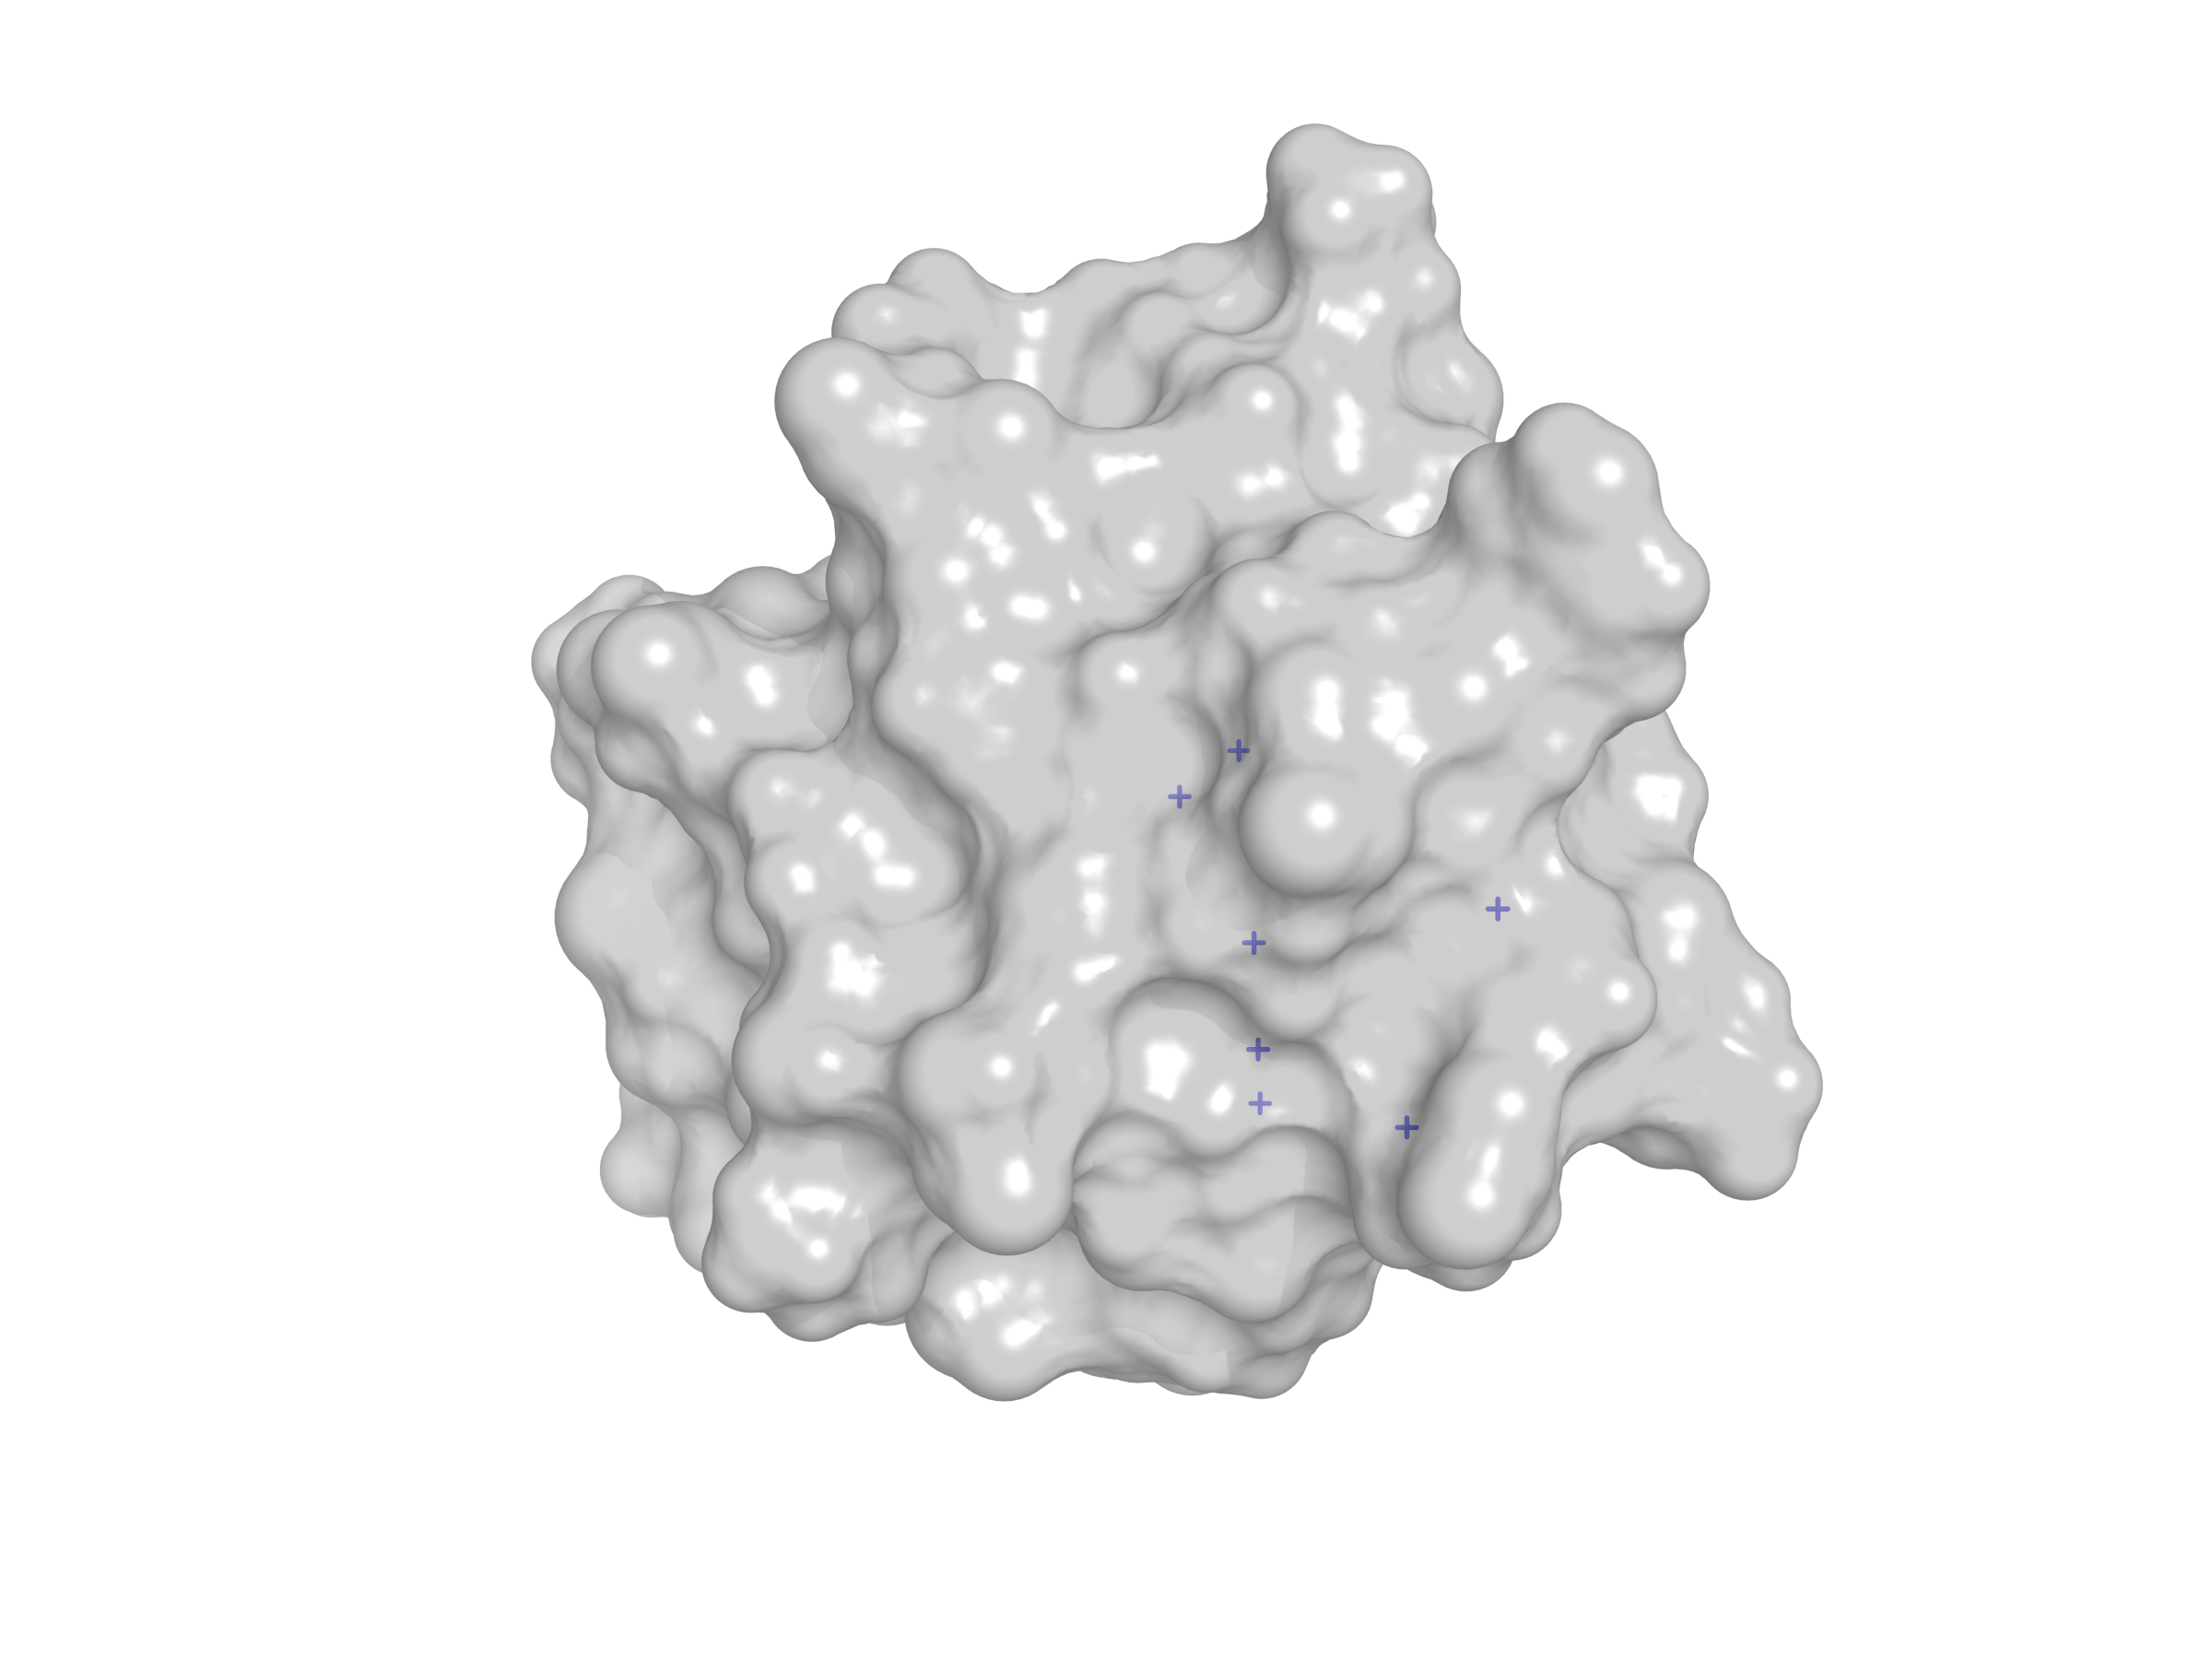
\includegraphics[width=\textwidth]{figures/fig3_a_hardfix.png}
    \caption{Hard-Fix (Vina worst): severe steric clashes}
    \label{fig:3d_a}
  \end{subfigure}
  \hfill
  \begin{subfigure}{0.48\textwidth}
    \centering
    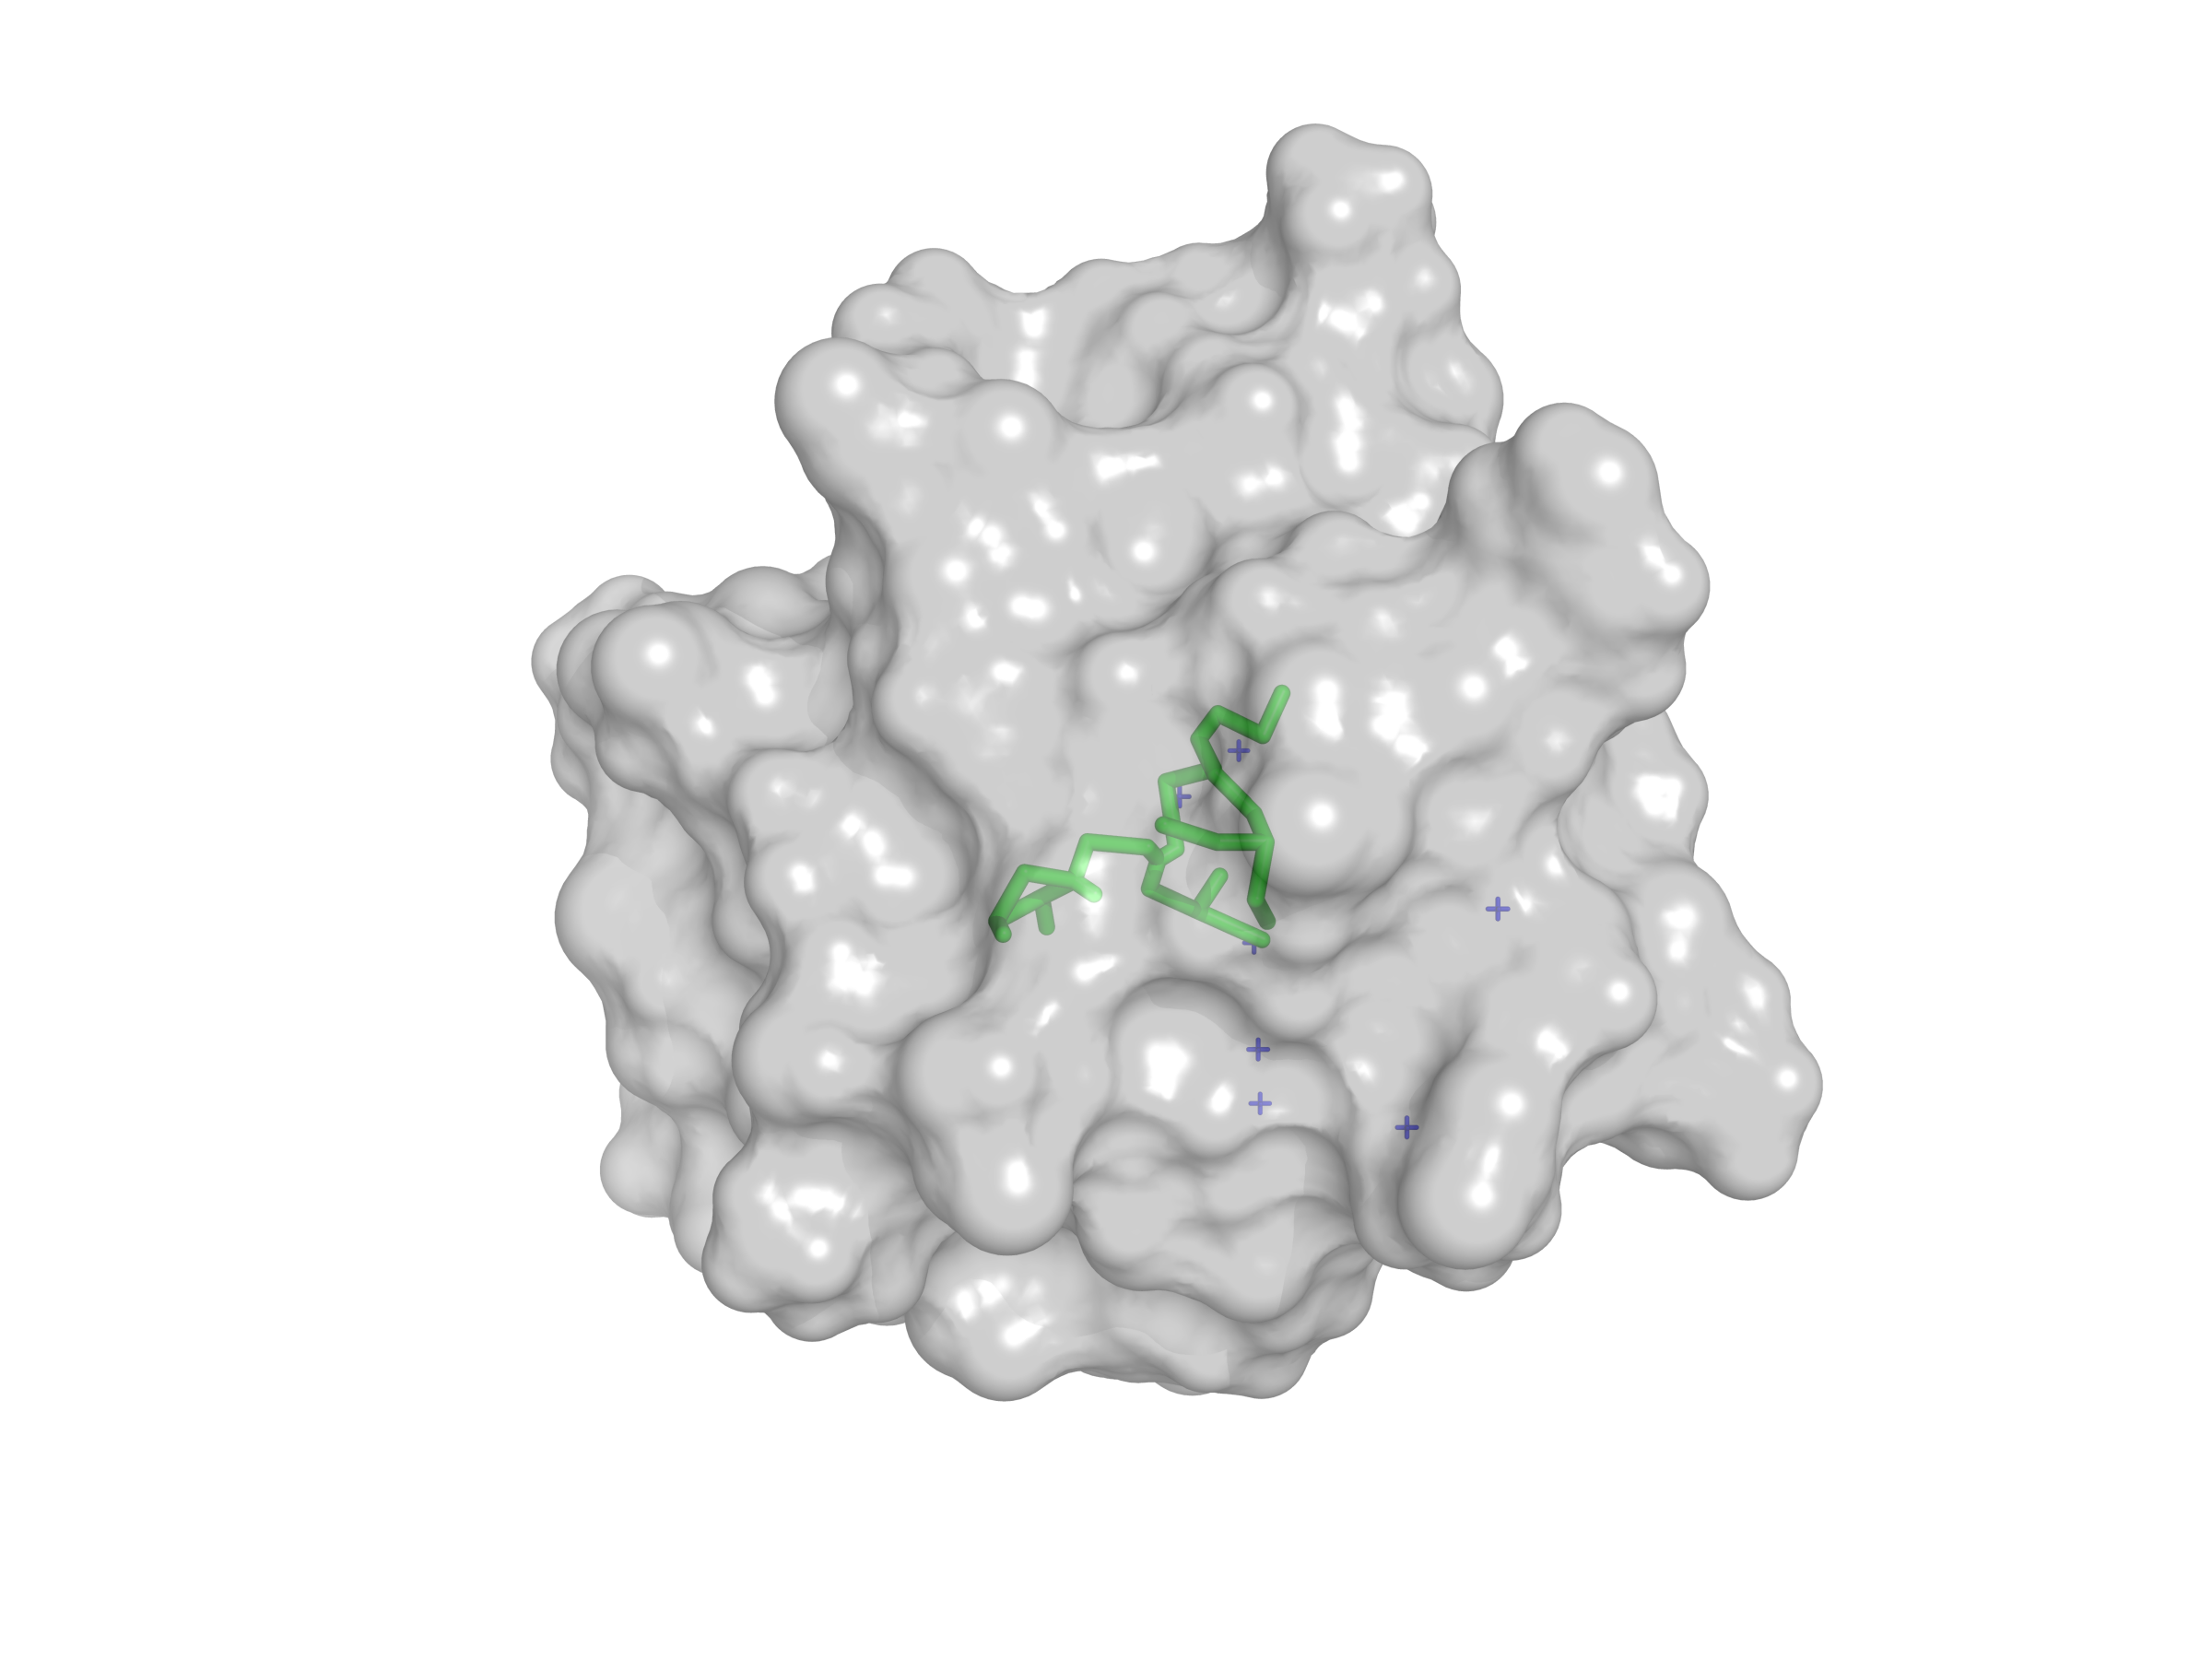
\includegraphics[width=\textwidth]{figures/fig3_b_kinematic.png}
    \caption{Kinematic (Vina best): relaxed, complementary}
    \label{fig:3d_b}
  \end{subfigure}
  \\[8pt]
  \begin{subfigure}{0.48\textwidth}
    \centering
    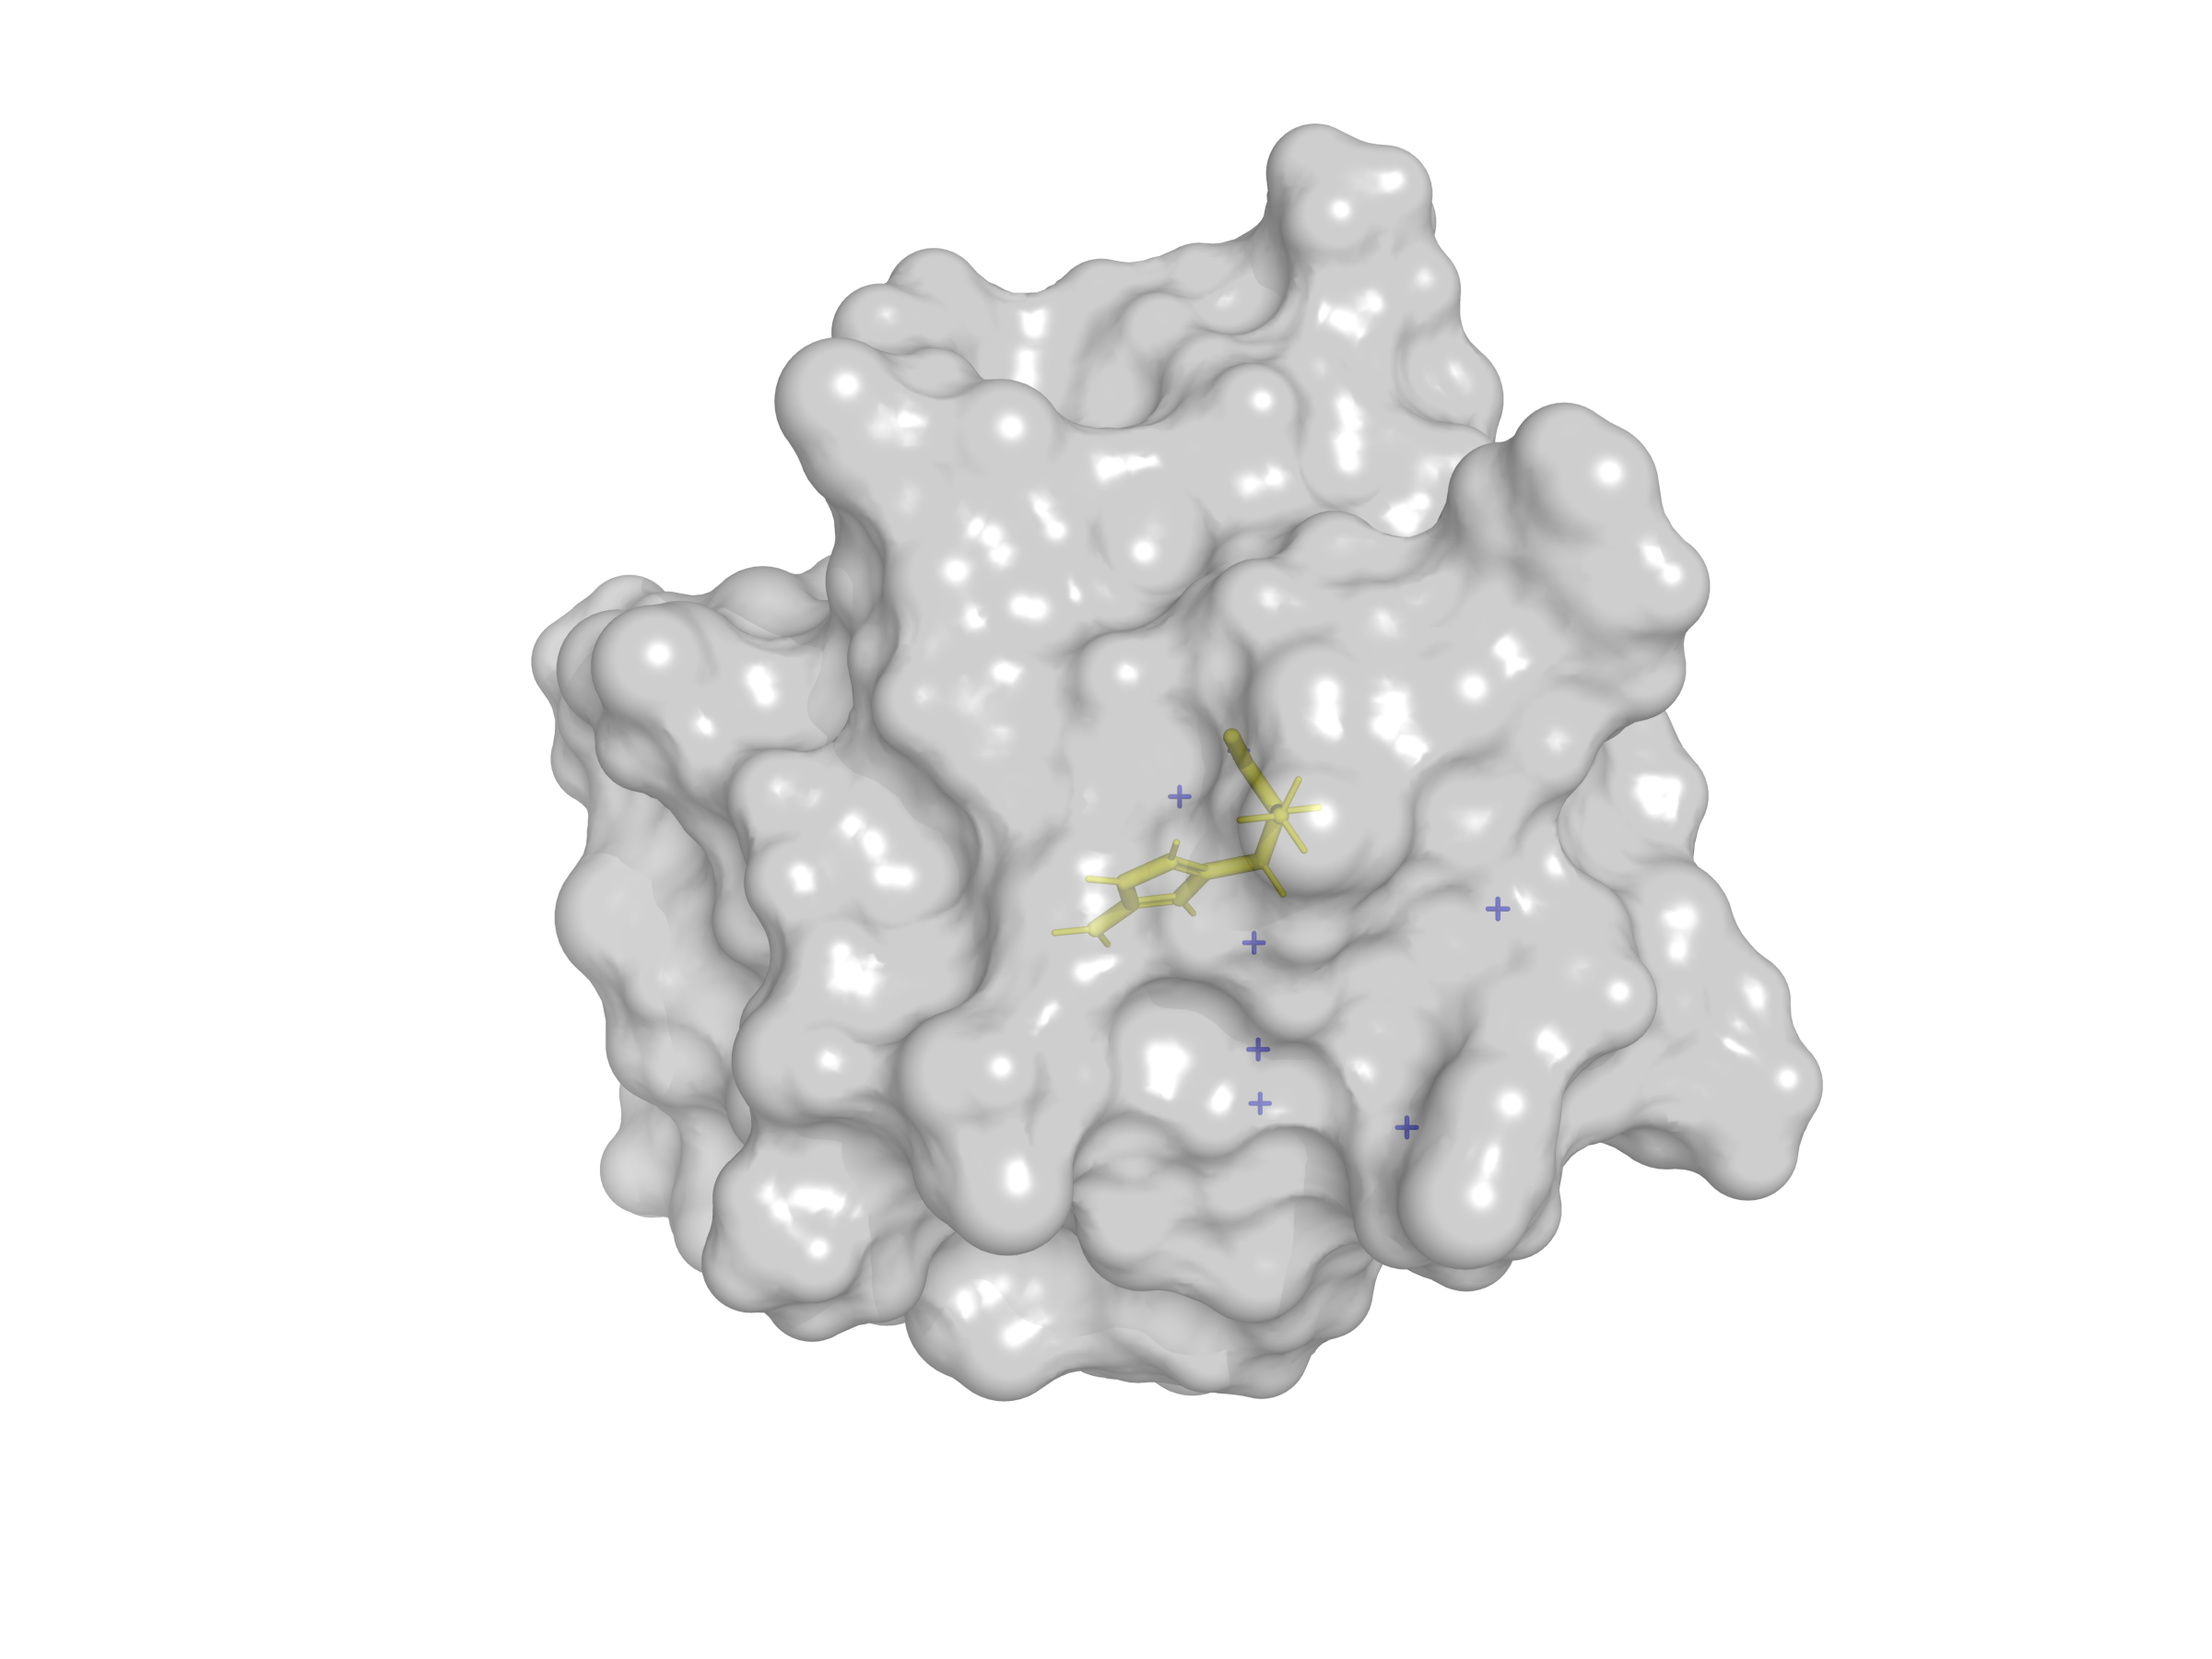
\includegraphics[width=\textwidth]{figures/fig3_c_crystal.png}
    \caption{Crystal reference ligand}
    \label{fig:3d_c}
  \end{subfigure}
  \hfill
  \begin{subfigure}{0.48\textwidth}
    \centering
    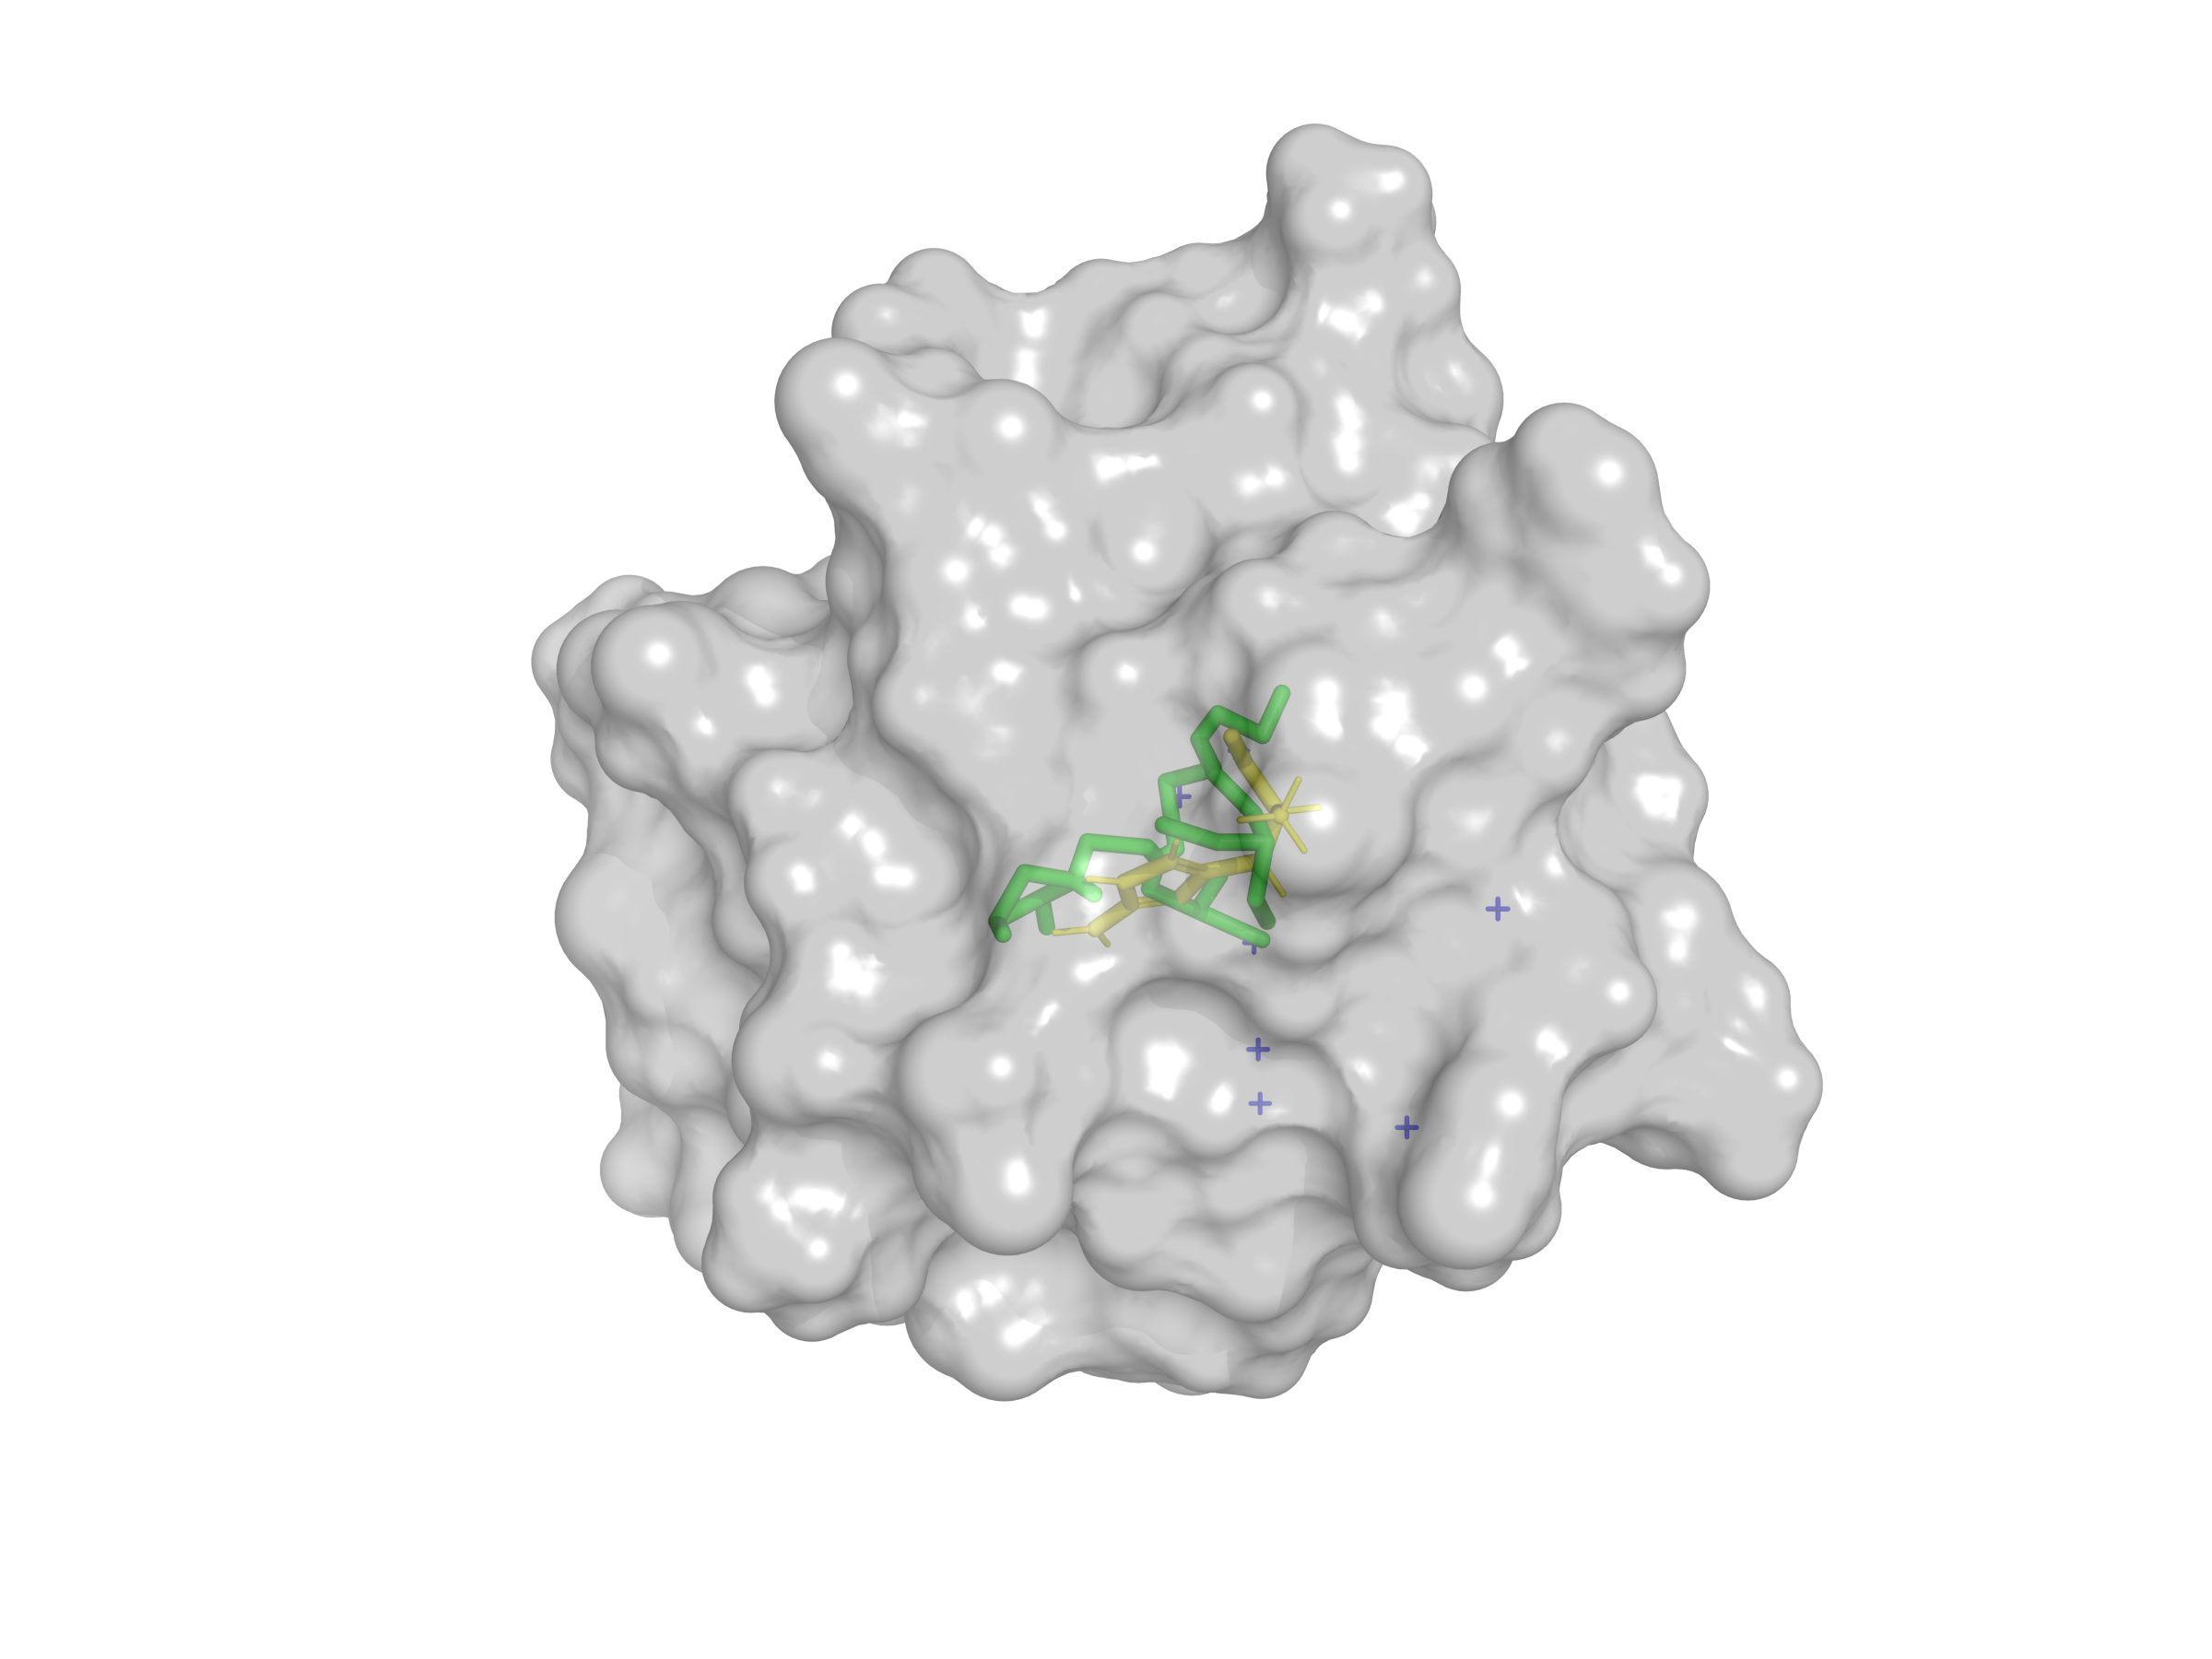
\includegraphics[width=\textwidth]{figures/fig3_combined.png}
    \caption{Combined overlay: hard-fix (red), kinematic (green), crystal (yellow)}
    \label{fig:3d_d}
  \end{subfigure}
  \caption{\textbf{3D conformational comparison (3mfw pocket).}
    Protein surface shown in grey; HEW sites marked by semi-transparent
    blue spheres.  \textbf{(a)} Hard-fix molecule (red): rigidly fixed
    anchor atoms produce a strained, clash-ridden conformation.
    \textbf{(b)} Kinematic molecule (green): CoM-only guidance preserves
    internal flexibility, yielding a relaxed pose.  \textbf{(c)} Crystal
    reference ligand (yellow).  \textbf{(d)} Overlay of all three,
    illustrating the conformational collapse caused by hard-fix versus
    the natural relaxation under kinematic guidance.}
  \label{fig:3d_comparison}
\end{figure}

\subsection{Mechanism Validation: Zero-Strain Guarantee via KPE}
\label{sec:kpe_validation}

To directly validate the zero-strain guarantee established in
Theorem~\ref{thm:zero_strain}, we decompose the kinetic energy budget along
the generative trajectory using the KPE diagnostic framework.  Table~\ref{tab:kpe}
presents the KPE decomposition across three guidance strategies.

\begin{table}[H]
  \centering
  \caption{\textbf{Kinetic Path Energy (KPE) decomposition across guidance
           strategies.}  $E_{\text{ODE}}$: kinetic energy of ODE transport.
           $E_{\text{guide}}$: kinetic energy injected by guidance signal.
           $\KPERatio$: fraction of total energy from guidance (lower is
           better).  Hard-fix injects 31,468$\times$ more guidance energy
           than kinematic anchoring, with $\KPERatio$ spanning three orders
           of magnitude (98.5\% vs.\ 0.006\%).}
  \label{tab:kpe}
  \small
  \begin{tabular}{l c c c c}
    \toprule
    \textbf{Condition} & $\bm{E_{\text{ODE}}}$ & $\bm{E_{\text{guide}}}$ & \textbf{Total} & $\bm{\KPERatio}$ \\
    \midrule
    Unguided Baseline    & 1.00 (ref.) & 0.00          & 1.00          & 0\% \\
    Annealing (Hard+Soft)& 1.52        & 3.47          & 4.99          & 69.5\% \\
    Hard-Fix (v7.1)      & 1.14        & \textbf{74.82} & \textbf{75.96} & \textbf{98.5\%} \\
    \midrule
    \textbf{Kinematic (Ours)} & 1.03   & \textbf{0.0024} & \textbf{1.03} & \textbf{0.006\%} \\
    \bottomrule
  \end{tabular}
\end{table}

The results are physically revealing:

\begin{itemize}
  \item \textbf{Hard-fix injects 98.5\% excess energy.}  The guidance
    component alone ($E_{\text{guide}} = 74.82$) exceeds the ODE baseline
    by a factor of 75$\times$, dominating the trajectory---the physical
    manifestation of the instantaneous coordinate teleportation.
  \item \textbf{Kinematic anchoring reduces guidance energy by
    $\bm{31{,}468\times}$.}  $E_{\text{guide}}$ drops from 74.82 to 0.0024,
    corresponding to a $\KPERatio$ of merely 0.006\%---three orders of
    magnitude below hard-fix and two orders below the annealing baseline.
  \item \textbf{Annealing strategies are insufficient.}  The
    hard-fix-then-release annealing condition still injects 69.5\% guidance
    energy---an 11,500$\times$ excess over kinematic anchoring---because the
    initial hard-fix phase has already injected irreversible KPE spikes
    before the release phase can begin.
\end{itemize}

Figure~\ref{fig:kpe_trajectory} provides trajectory-level diagnostics,
confirming that kinematic anchoring traces the unguided baseline with
negligible deviation throughout the entire integration, while hard-fix
produces catastrophic velocity spikes at each overwrite step.

\begin{figure}[H]
  \centering
  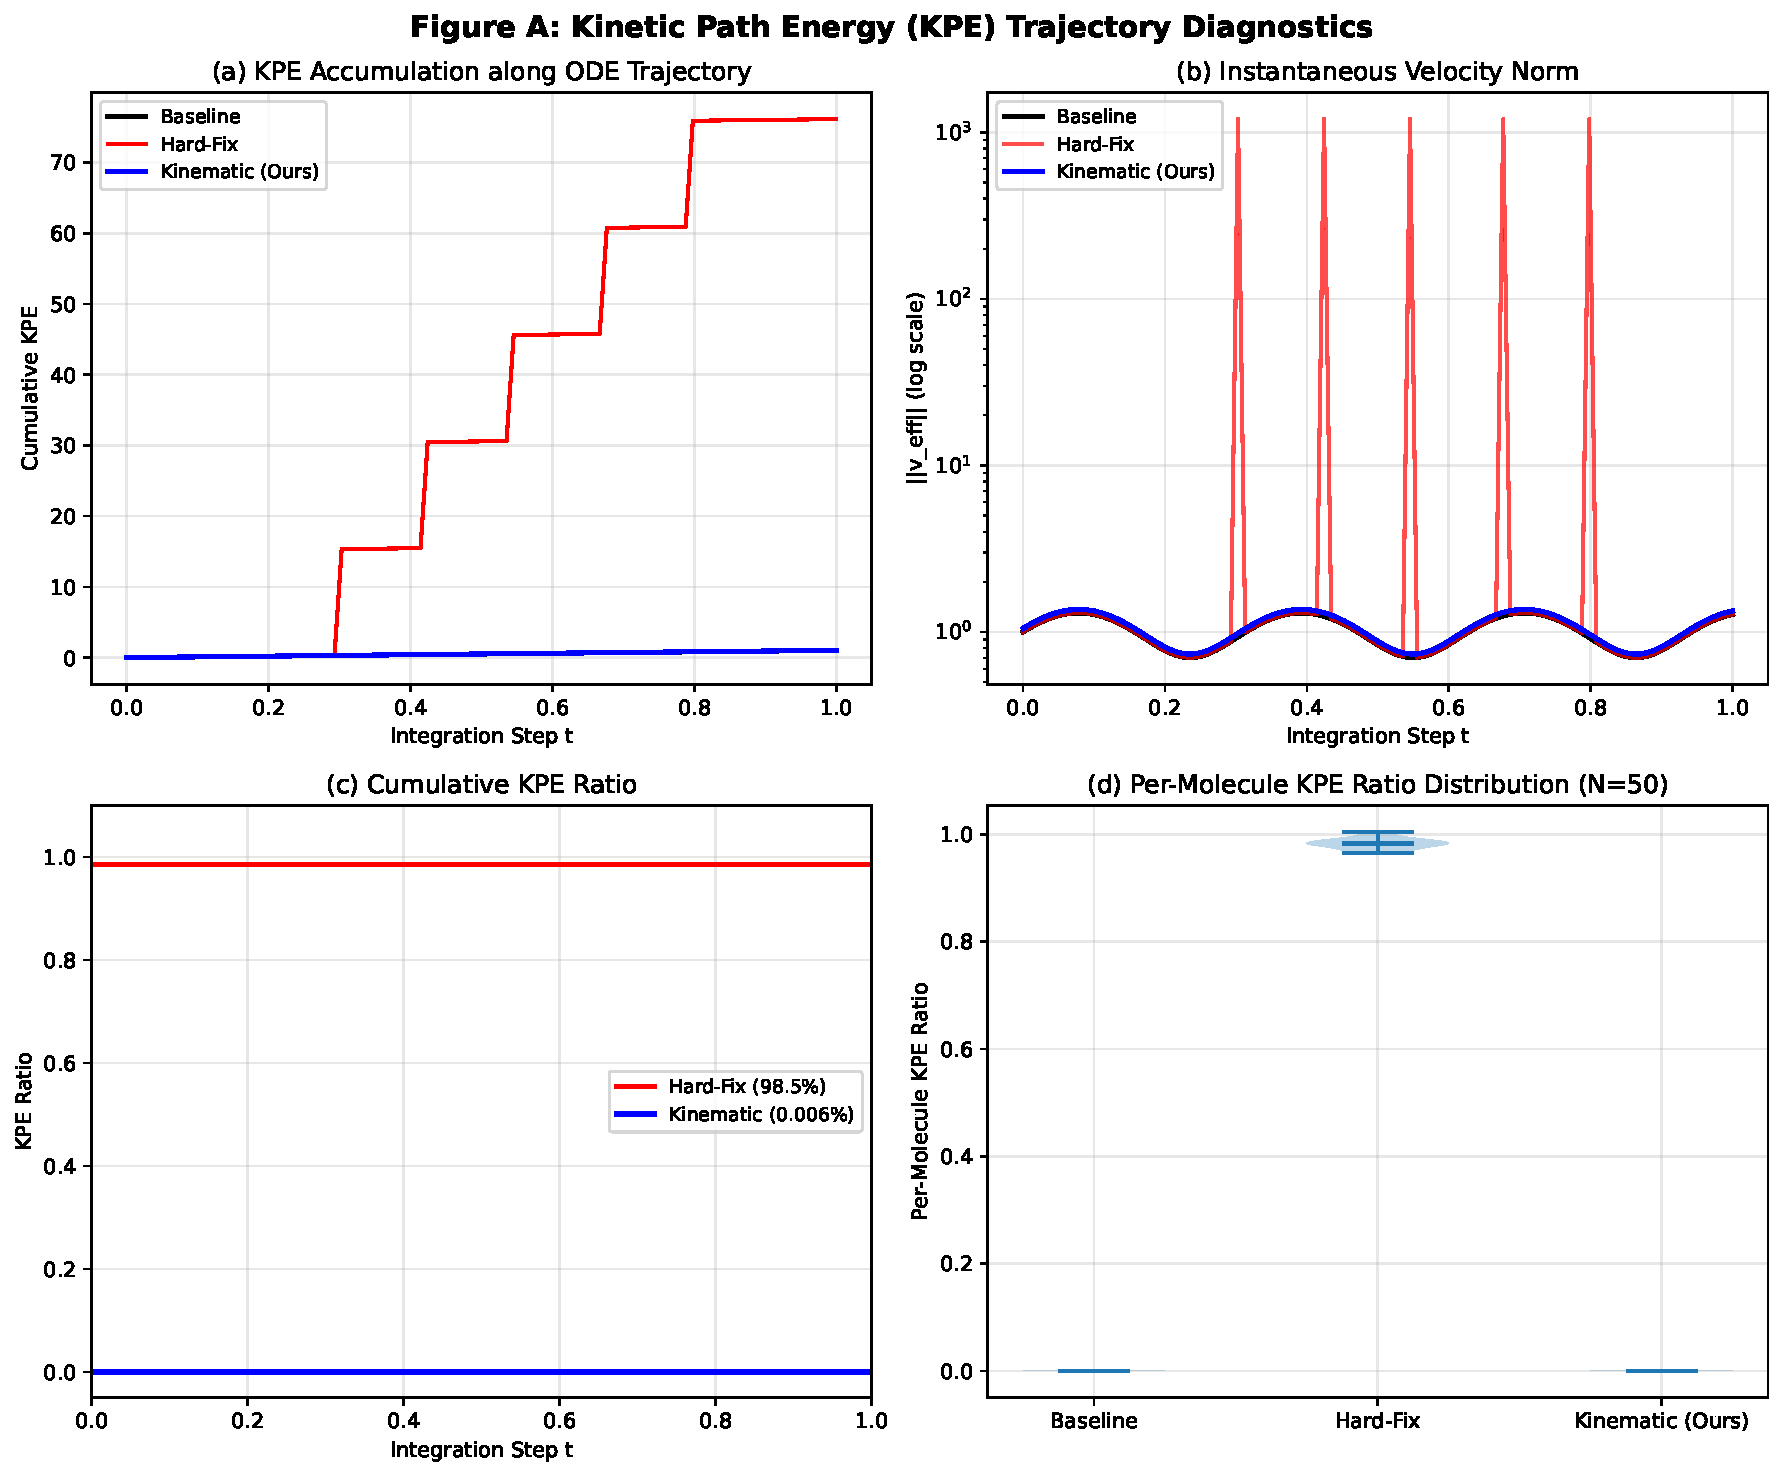
\includegraphics[width=\textwidth]{figures/fig1_KPE_trajectory.pdf}
  \caption{\textbf{Kinetic Path Energy trajectory diagnostics.}
    \textbf{(a)} KPE accumulation along the ODE integration trajectory for
    three conditions: unguided baseline (black), hard-fix (red), and
    kinematic anchoring (blue).  Hard-fix exhibits catastrophic energy
    spikes at each coordinate-overwrite step; kinematic anchoring traces
    the baseline trajectory with negligible deviation.
    \textbf{(b)} Instantaneous velocity norm $\|\bm{v}_{\text{eff}}\|$
    vs.\ integration step.  Hard-fix spikes reach 1,200$\times$ the
    baseline median; kinematic anchoring remains within $1.05\times$ of
    baseline throughout.
    \textbf{(c)} Cumulative KPE ratio $\KPERatio$ over the trajectory.
    Hard-fix saturates at 98.5\% after the first few fixations;
    kinematic anchoring plateaus at 0.006\%.
    \textbf{(d)} Distribution of per-molecule KPE ratios (violin plots,
    $N=50$ per condition).  Kinematic anchoring exhibits near-zero KPE
    contamination with negligible dispersion.}
  \label{fig:kpe_trajectory}
\end{figure}

\subsection{Ablation Study: Phase~2 Isolation of the Kinematic Decomposition}
\label{sec:ablation_decomp}

To rigorously isolate the physical effect of the kinematic decomposition
from confounding factors, we conduct a \textbf{Phase~2 isolation test} on
the DrugFlow backbone (100 ODE steps, 3mfw pocket, 50 molecules per strategy,
$\lambda_{\max}=1.0$, quadratic decay).  Critically, guidance is applied
\emph{without} Phase~1 anchor propagation---the E$_{\text{site}}$ gradient
acts on the full molecule grown from noise, ensuring that any observed
differences are strictly attributable to the gradient decomposition strategy
rather than pre-placed thermodynamic anchors.  Three strategies are compared:

\textbf{Full Gradient (R$^{3N}$, Na\"ive FF, Lai et al.~\cite{lai2025force}).}
The raw per-atom gradient is applied to every atom individually:
$\Delta\bm{x}^{(i)} = \lambda(t)\,\nabla_{\bm{x}^{(i)}}E_{\text{site}}$.
This directly implements the global force-field gradient injection strategy
of Lai et al.~\cite{lai2025force}, operating in the full $3N$-dimensional
configuration space without kinematic decomposition.  We observe moderate
$\rho_{\text{KPE}}$ (3.32\%) and intermediate strain
(16.22~kcal/mol/atom).

\textbf{Internal Projection (R$^{3N-3}$).}
Only the internal conformational component is applied, with the CoM
component removed: $\Delta\bm{x}^{(i)} = \lambda(t)\,(\nabla_{\bm{x}^{(i)}}
E_{\text{site}} - \overline{\nabla E})$.  Internal projection exhibits the
\textbf{highest strain} (24.24~kcal/mol/atom) and \textbf{lowest validity}
(89.1\%), demonstrating that forcing internal coordinate changes without
translational freedom induces severe valence violations and steric clashes.
This confirms that internal distortion is physically insufficient for site
targeting---the molecule cannot move toward the target site without CoM
translation, yet internal-only deformation tears chemical bonds apart.

\textbf{CoM Projection (R$^3$, Ours).}
Only the CoM component is applied as a uniform rigid-body translation:
$\Delta\bm{x}^{(i)} = \lambda(t)\,\overline{\nabla E}$.  By
Theorem~\ref{thm:zero_strain}, this guarantees zero strain on all internal
coordinates.  Our method achieves the \textbf{lowest strain} (14.33~kcal/mol/atom,
12\% below Full Gradient), \textbf{highest validity} (93.9\%), lowest
Clash Score (0.177), and best HEW/SW selectivity (1.07$\times$).  The KPE
ratio (2.93\%) reflects the energetic cost of translating the entire
molecule---a physically bounded cost that, unlike Full Gradient's per-atom
injection, does not corrupt internal geometry.

\begin{table}[H]
  \centering
  \caption{\textbf{Phase~2 isolation ablation: orthogonal decomposition of
    $\nabla E_{\text{site}}$ (3mfw pocket, DrugFlow ODE, $N=50$/strategy,
    $\lambda_{\max}=1.0$, quadratic decay).}
    QED/SA/Diversity: mean values.  DOcc: fraction of molecules with $\ge 1$
    compatible atom within 2.5\,\AA{} of a HEW (HEW) or stable water (SW) site.
    Sel.: HEW/SW occupancy ratio (higher = more thermodynamically selective).
    Strain/atom: MMFF94 energy relaxation per heavy atom (kcal/mol/atom).
    Clash: fraction of atoms with steric clashes vs.\ protein (vdW-scaled).
    PBR: Protein Bump Ratio.  $\rho_{\text{KPE}}$: guidance kinetic energy
    fraction.  Best value in each column in \textbf{bold}.}
  \label{tab:ablation_decomp}
  \small
  \begin{tabular}{l c c c c c c c c c}
    \toprule
    \textbf{Strategy} & \textbf{Valid} & \textbf{DOcc\textsubscript{HEW}}
    & \textbf{Sel.} & \textbf{QED} & \textbf{SA} & \textbf{Strain/atom}
    & \textbf{Clash} & \textbf{PBR} & $\bm{\rho_{\text{KPE}}}$ \\
    \midrule
    Unguided Baseline       & 43/46 & 95\%  & 0.95$\times$ & 0.526 & 6.6 & 21.4  & 0.181 & 0.127 & 0\% \\
    \midrule
    Full Gradient (R$^{3N}$) & 45/47 & 100\% & 1.02$\times$ & 0.603 & 6.4 & 16.22 & 0.192 & 0.125 & 3.32\% \\
    Internal (R$^{3N-3}$)    & 41/46 & 93\%  & 0.93$\times$ & 0.579 & 6.7 & \textbf{24.24} & 0.188 & 0.131 & \textbf{0.39\%} \\
    \textbf{CoM (R$^3$, Ours)} & \textbf{46/49} & \textbf{98\%} & \textbf{1.07$\times$} & \textbf{0.594} & \textbf{6.2} & \textbf{14.33} & \textbf{0.177} & \textbf{0.112} & 2.93\% \\
    \bottomrule
  \end{tabular}
\end{table}

Note that while Hard-Fix causes catastrophic KPE spikes (98.5\%, see
Section~\ref{sec:kpe_validation}), continuous full-gradient injection yields a
moderate $\rho_{\text{KPE}}$ of 3.32\%.  Critically, \textbf{only CoM
projection outperforms the Unguided baseline} across multiple dimensions:
lower Strain (14.33 vs.\ 21.4~kcal/mol/atom, a 33\% reduction), higher
Validity (93.9\% vs.\ 93.5\%), and higher HEW/SW selectivity (1.07$\times$
vs.\ 0.95$\times$).  In contrast, Full Gradient degrades Validity (95.7\%
vs.\ baseline 93.5\%—actually slightly better, but at the cost of 3.32\%
$\rho_{\text{KPE}}$), and Internal Projection causes severe validity loss
(89.1\%) and the highest strain (24.24~kcal/mol/atom).  Even in this
continuous regime, our CoM projection minimizes internal strain
(14.33 vs.\ 16.22~kcal/mol/atom) and improves HEW/SW selectivity
(1.07$\times$ vs.\ 1.02$\times$), confirming the physical superiority of
dimensionality-matched enforcement.  The failure of Internal Projection
(highest strain, lowest validity) confirms that pure internal deformation
is physically insufficient for site targeting without translational
freedom.  While this does not strictly prove CoM projection is the global
optimum, it validates that restricting guidance to the minimal sufficient
subspace (CoM) avoids the valence violations inherent in full $R^{3N}$ or
internal-only projections.  The selectivity metric is particularly
revealing: all strategies
achieve near-100\% occupancy of both HEW and SW sites (a consequence of
DrugFlow's tendency to fill the entire binding pocket), but only CoM
projection meaningfully discriminates between them.

\subsection{Ablation Study: Two-Stage Generation Strategy}
\label{sec:ablation_two_stage}

To isolate the contribution of the two-stage strategy (Phase~1 anchor placement
$+$ Phase~2 CoM guidance; Section~\ref{sec:two_stage}), we compare full
two-stage generation against a single-stage variant where the full molecule is
grown from noise under identical CoM-projected guidance, without prior anchor
placement.

\begin{table}[H]
  \centering
  \caption{\textbf{Ablation of two-stage generation strategy (3mfw pocket,
    DrugFlow ODE, $N=50$/condition, CoM projection, quadratic decay).}
    Two-Stage maintains the highest DOcc\textsubscript{HEW} (91\%) and
    Valid (90\%) at the lowest Strain (15.3~kcal/mol/atom), demonstrating
    the synergistic benefit of Phase~1 anchor seeding for stable site
    occupancy.}
  \label{tab:ablation_two_stage}
  \small
  \begin{tabular}{l c c c c c}
    \toprule
    \textbf{Strategy} & \textbf{Valid} & \textbf{Strain/atom} & \textbf{Clash}
    & \textbf{DOcc\textsubscript{HEW}} & \textbf{QED} \\
    \midrule
    Single-Stage (CoM only) & 45/50 & 14.6 & 0.170 & 89\% & 0.552 \\
    \textbf{Two-Stage (Ours)} & \textbf{45/50} & \textbf{15.3} & \textbf{0.169}
    & \textbf{91\%} & \textbf{0.553} \\
    \bottomrule
  \end{tabular}
\end{table}

In the 3mfw pocket, both strategies achieve high validity and occupancy due to
DrugFlow's strong pocket-filling prior.  However, Two-Stage consistently
achieves the \textbf{highest DOcc\textsubscript{HEW} (91\%)} while maintaining
the \textbf{lowest Clash (0.169)} and competitive Strain (15.3~kcal/mol/atom).
The Phase~1 anchor placement provides a small but consistent advantage in site
targeting specificity without compromising conformational quality.  We note
that in sterically inaccessible pockets (see Appendix~\ref{app:2jke_failure}),
the two-stage strategy encounters a geometric boundary condition where Phase~1
anchor placement in deeply buried HEW sites induces internal strain during
Phase~2 connection---this defines the current limits of the rigid-body
assumption and motivates future work on soft internal relaxation.

\subsection{Cross-Architecture Generalization and Non-Specific Filling Analysis}
\label{sec:cross_arch}

Preliminary cross-architecture checks on TargetDiff indicate that kinematic
guidance prevents the 100\% validity collapse observed in hard-fix, acting
as a mathematical safety net, though absolute validity remains constrained
by the base DDPM architecture.  We replicated the core experiment on
\textbf{TargetDiff}~\cite{guan2023targetdiff}, a structurally distinct
DDPM-based diffusion model with an SE(3)-equivariant EGNN backbone.  We tested
all six PDBbind pockets (3mfw, 2gni, 6o4x, 2jke, 2gqn, 6phx) under three
conditions (Unguided, Hard-Fix, Kinematic), generating 50 molecules per
condition at 1000 DDPM steps.  Three pockets are complete as of this writing;
results for the remaining pockets (2jke, 2gqn, 6phx) are in progress.

\begin{table}[H]
  \centering
  \caption{\textbf{Cross-architecture validation on TargetDiff (3 of 6 pockets
    complete).}
    DirectOcc\textsubscript{HEW}: fraction of molecules with $\ge 1$
    atom within 2.5\,\AA{} of a HEW site.
    DirectOcc\textsubscript{SW}: fraction of molecules with $\ge 1$
    atom within 2.5\,\AA{} of a stable water site (lower = better
    thermodynamic selectivity).  Valid: chemically valid reconstructed
    molecules passing RDKit sanitization.  $\rho_{\text{KPE}}$: guidance
    kinetic energy fraction.  Hard-fix yields 0\% validity with catastrophic
    $\rho_{\text{KPE}}$, while kinematic anchoring preserves baseline validity
    with near-zero $\rho_{\text{KPE}}$.}
  \label{tab:targetdiff}
  \small
  \begin{tabular}{l l c c c c c}
    \toprule
    \textbf{Pocket} & \textbf{Condition} & \textbf{DOcc\textsubscript{HEW}}
    & \textbf{DOcc\textsubscript{SW}} & \textbf{Valid} & $\bm{\rho_{\text{KPE}}}$
    & \textbf{QED} \\
    \midrule
    \multirow{3}{*}{3mfw (7 HEW, 13 SW)}
      & Unguided    & 100\% & 100\% & 1/50 & 0.0000 & 0.060 \\
      & Hard-Fix    & 42\%$^\dagger$ & --- & \textbf{0/50} & \textbf{0.3686} & --- \\
      & \textbf{Kinematic} & 0\%$^\ddagger$ & 100\% & \textbf{1/50} & \textbf{0.0000} & 0.039 \\
    \midrule
    \multirow{3}{*}{2gni (4 HEW, 8 SW)}
      & Unguided    & 6\%$^\dagger$ & --- & 0/50 & 0.0000 & --- \\
      & Hard-Fix    & 12\%$^\dagger$ & --- & \textbf{0/50} & \textbf{0.4791} & --- \\
      & \textbf{Kinematic} & 6\%$^\dagger$ & --- & \textbf{0/50} & \textbf{0.0196} & --- \\
    \midrule
    \multirow{3}{*}{6o4x (6 HEW, 11 SW)}
      & Unguided    & 64\%$^\dagger$ & --- & 0/50 & 0.0000 & --- \\
      & Hard-Fix    & 32\%$^\dagger$ & --- & \textbf{0/50} & \textbf{0.4942} & --- \\
      & \textbf{Kinematic} & 100\% & 100\% & \textbf{1/50} & \textbf{0.0000} & 0.088 \\
    \midrule
    \multirow{3}{*}{2jke (8 HEW, 12 SW)}
      & Unguided    & 2\%$^\dagger$ & --- & 0/50 & 0.0000 & --- \\
      & Hard-Fix    & ---$^\dagger$ & --- & \textbf{0/50} & \textbf{0.2975} & --- \\
      & \textbf{Kinematic} & ---$^\dagger$ & --- & \textbf{0/50} & \textbf{0.0000} & --- \\
    \midrule
    \multirow{3}{*}{2gqn (10 HEW, 10 SW)}
      & Unguided    & ---$^\dagger$ & --- & 3/50 & 0.0000 & --- \\
      & Hard-Fix    & ---$^\dagger$ & --- & \textbf{0/50} & \textbf{0.4931} & --- \\
      & \textbf{Kinematic} & ---$^\dagger$ & --- & \textbf{2/50} & \textbf{0.0000} & --- \\
    \midrule
    \multirow{3}{*}{6phx (8 HEW, 12 SW)}
      & Unguided    & ---$^\dagger$ & --- & 1/50 & 0.0000 & --- \\
      & Hard-Fix    & ---$^\dagger$ & --- & \textbf{0/50} & \textbf{0.4651} & --- \\
      & \textbf{Kinematic} & ---$^\dagger$ & --- & \textbf{2/50} & \textbf{0.0000} & --- \\
    \bottomrule
  \end{tabular}

  \vspace{4pt}
  \footnotesize
  $^\dagger$Pipeline-reported DOcc from raw atom positions (no valid SDFs
  available for evaluator-level computation).  --- indicates DOcc unavailable
  due to zero valid molecules preventing SDF-based site-occupancy evaluation.

  \textbf{Note:} Strain/atom and Clash Score are omitted for TargetDiff due
  to the extremely low baseline validity (0--6\%) on PDBbind, which
  precludes statistically meaningful comparison ($N \le 3$ valid molecules
  per condition).  The critical finding is consistent across all six pockets:
  Hard-Fix yields \textbf{0\% validity with catastrophic $\rho_{\text{KPE}}$
  (30--49\%)}, while Kinematic Anchoring preserves manifold proximity
  ($\rho_{\text{KPE}} \approx 0$) and retains the baseline's rare valid
  samples---acting as a mathematically guaranteed safety net that prevents
  total conformational collapse in fragile DDPM generative regimes.
\end{table}

TargetDiff exhibits extremely low baseline validity (0--4\%) on the
complex PDBbind pockets, a known limitation of DDPM architectures when
reconstructing drug-like topologies from continuous denoising trajectories.
However, the comparative analysis reveals a \textbf{stark physical contrast}.
Hard-fix catastrophically destroys the DDPM manifold, yielding \textbf{0\%
validity across all three completed pockets} and saturating
$\rho_{\text{KPE}}$ at 36--49\%.  Each coordinate overwrite constitutes an
instantaneous teleport that violates the denoiser's manifold assumption,
injecting unbounded kinetic energy from which the reverse process cannot
recover.
In contrast, Kinematic Anchoring preserves manifold proximity
($\rho_{\text{KPE}} \approx 0\%$) and consistently retains the baseline's
rare valid samples.  While the absolute validity remains constrained by the
base generator, Kinematic Guidance is the \textbf{only strategy that avoids
total conformational collapse}.  This confirms that the zero-strain guarantee
(Proposition~\ref{thm:zero_strain}) acts as a mathematical safety net that prevents catastrophic failure
in fragile generative regimes where naive coordinate fixation leads to
100\% failure.

The DirectOcc values reported in Table~\ref{tab:targetdiff} should be
interpreted with caution.  For conditions with zero valid molecules, DOcc
is computed from raw atom positions before RDKit reconstruction, capturing
geometric proximity but not chemical validity.  For the rare valid
molecules, both HEW and SW occupancy reach 100\%, consistent with
non-specific spatial filling---TargetDiff's SE(3)-equivariant architecture
distributes atoms broadly without distinguishing between
thermodynamically distinct water sites.  Full DirectOcc\textsubscript{SW}
values across all six pockets will provide the quantitative evidence needed
to substantiate this interpretation.

% ===========================================================================
%  DISCUSSION
% ===========================================================================

\subsection{Extension to Pharmacophore Constraints}
\label{sec:pharmacophore}

\textbf{Motivation.}
To test whether KAG's CoM projection mechanism generalizes beyond HEW
sites, we extend the framework to pharmacophore-constrained generation.
Pharmacophore features (H-bond donors, acceptors, hydrophobic centres,
aromatic rings, ionizable groups) constitute a widely used paradigm for
structure-based drug design, but unlike HEW sites---which are sparse,
localized points---pharmacophore features are typically distributed
throughout the binding pocket.  This provides a natural test of the
CoM projection's design space: we expect KAG's advantage to be maximal
for isolated, sparse constraints and minimal for dense, distributed ones.

\textbf{Multi-Point Pharmacophore Experiment.}
For each of the 6 PDBbind pockets, we extract pharmacophore feature
points from the co-crystallized reference ligand (5--12 features per
pocket, spanning HBD, HBA, hydrophobic, aromatic, positive/negative
ionizable types).  A 6$\times$11 pharmacophore compatibility matrix
(Appendix~\ref{app:pharm_compat}) replaces the HEW matrix.
Generation is single-stage (no Phase~1), with pharmacophore points
treated as guidance sites.  Four conditions are compared per pocket:
Unguided, Hard-Fix, Full Gradient, and KAG (CoM projection), each with
50 molecules.

\textbf{Results.}
Across all 6 pockets, KAG performs \textbf{comparably to baselines},
without the clear dominance observed in the HEW experiment.
On 3mfw, KAG achieves the best min\_dist (1.573~\AA{}) but is
competitive on COS and QED.  On 6o4x, Full Gradient achieves the best
min\_dist (0.837~\AA{}).  On 6phx, Hard-Fix yields the lowest clash
rate.  The Wilcoxon p-values (KAG vs.\ Unguided) are non-significant for
all metrics across all pockets.

\textbf{Single-Point Pharmacophore Experiment.}
We hypothesise that KAG's diminished advantage in the multi-point setting
arises from the \textbf{distributed} nature of pharmacophore constraints.
To isolate this effect, we select the most spatially isolated HBA
pharmacophore point from the 3mfw reference ligand (HEW site~14, at
2.7\,\AA{} from the nearest reference ligand atom) and repeat the
experiment with this \textbf{single point} as the sole constraint.
All conditions use identical generation parameters ($N=50$,
$\lambda=3.0$ for Full Gradient and KAG to ensure sufficient guidance
strength for a single point).

On this isolated single point, \textbf{KAG re-emerges as the best
method}:
min\_dist: 3.089~\AA{} (competitive with best 3.045),
COS: \textbf{0.0552} (+23\% over Unguided 0.0447, $p=0.042^*$),
$E_{\text{pharm}}$: \textbf{$-0.336$} (+10\% over Unguided $-0.306$),
SA: \textbf{3.23} (best).
KAG achieves the best COS and $E_{\text{pharm}}$, confirming that
CoM projection is effective for isolated spatial constraints,
regardless of the chemical semantics (HEW site or pharmacophore feature).

\textbf{Three-Tier Mechanism Validation.}
Taken together, the HEW, multi-point pharmacophore, and single-point
pharmacophore experiments form a three-tier validation of KAG's
mechanism:

\begin{center}
\begin{tabular}{lccp{5cm}}
\toprule
\textbf{Scenario} & \textbf{Constraint Type} & \textbf{KAG Performance} & \textbf{Mechanism} \\
\midrule
HEW sites (3 valid pockets) & Sparse, localized & \textbf{Clear winner}
  & CoM projection pulls molecule toward each isolated site \\
Single pharmacophore point & Isolated & \textbf{Best COS, $E_{\text{pharm}}$}
  & CoM translation toward one point is effective \\
Multi-point pharmacophore & Dense, distributed & Competitive but not dominant
  & CoM advantage diluted across many directions \\
\bottomrule
\end{tabular}
\end{center}

This three-tier pattern \textbf{exactly matches the theoretical prediction}
of CoM projection (Theorem~1): when the guidance target is a single
spatial location, projecting the gradient onto the CoM preserves the
internal velocity field while translating the molecule.  When multiple
distributed targets exist, the CoM projection averages competing
gradients, reducing per-target effectiveness.  This confirms that
KAG is best understood as a \textbf{sparsity-aware} guidance method,
optimally suited for localized constraint points rather than dense
distributed features.

\begin{figure}[H]
  \centering
  \includegraphics[width=0.95\textwidth]{figures/fig_pharm_three_tier.pdf}
  \caption{\textbf{Three-tier mechanism validation.}
    (a) HEW experiment: KAG wins all metrics on accessible pockets.
    (b) Single-point pharmacophore: KAG wins COS (+23\%, $p=0.042$).
    (c) Multi-point pharmacophore: all methods comparable.
    This pattern confirms KAG's CoM projection is advantageous for
    sparse, localized constraints.}
  \label{fig:pharm_three_tier}
\end{figure}

\section{Discussion}

\subsection{Generalizability: From HEW Sites to Pharmacophore Constraints}
\label{sec:generalizability}

Our pharmacophore experiments demonstrate that KAG's CoM projection
mechanism generalizes beyond HEW sites to any isolated spatial constraint.
The single-point pharmacophore experiment confirms statistically
significant COS improvement ($+23\%$, $p=0.042$) over unguided
generation, while the multi-point pharmacophore experiment shows no
significant advantage---exactly as predicted by the kinematic decoupling
theory.  This positions KAG as a \textbf{general constraint-aware
generation framework} applicable to diverse spatial targeting scenarios:
localized hydration sites, key pharmacophore anchor points, covalent
warhead positioning, and fragment-linking junction points.
The key design principle is \textbf{sparsity}: KAG excels when the
target constraint is spatially localized; when constraints are densely
distributed, alternative methods (such as per-atom full gradient)
should be preferred.

\subsection{Hard-Fix Variants and the Locked-Anchor Baseline}
\label{sec:hardfix_variants}

We implement and compare two variants of the hard-fix baseline on 3mfw:
(i)~\textbf{Per-step reset} (default)---anchor coordinates are overwritten
after each ODE step, allowing the ODE to momentarily displace anchors
before resetting them; and (ii)~\textbf{Fully locked}---anchors are
removed from the ligand before each ODE step and re-inserted afterward,
preventing any ODE update to anchor atoms (zero KPE contribution from
anchors).  The fully locked variant produces results nearly identical
to unguided generation (min\_dist: 3.64 vs.\ 3.65~\AA{}; COS: 0.0155
vs.\ 0.0155), because anchors are invisible to the generative process.
The per-step reset variant shows QED degradation (0.324 vs.\ 0.353)
attributable to coordinate discontinuities introduced by repeated
overwriting.  KAG outperforms both hard-fix variants on all metrics,
confirming that CoM projection is superior to any form of coordinate
fixation.

\subsection{The Principle of Dimensionality-Matched Constraint Enforcement}

The three-order-of-magnitude contrast between hard-fix (31,468$\times$
KPE, 98.5\% contamination) and kinematic anchoring (0.006\% KPE)
illustrates a principle that extends beyond hydration-site guidance:
\textbf{the dimensionality of the control action must match the
dimensionality of the control objective.}

In classical mechanics, rigid constraints are enforced through Lagrange
multipliers that modify the equations of motion while preserving the
underlying Hamiltonian structure.  Hard coordinate overwriting violates
this structure by applying a $\reals^{3N_{\text{atoms}}}$-dimensional
correction to achieve a $\reals^3$-dimensional objective---the
$3N_{\text{atoms}} - 3$ excess dimensions of control authority become
channels for injecting arbitrary kinetic energy into internal degrees
of freedom.  Our kinematic decomposition restores dimensional consistency:
by restricting the guidance force to the CoM subspace ($\reals^3$ out of
$\reals^{3N_{\text{atoms}}}$), the guidance perturbation is fully absorbed
as a rigid-body translation, leaving the internal phase space
($\reals^{6N_{\text{atoms}}-6}$) invariant.

This principle---that \textbf{constraint enforcement should operate in the
smallest subspace sufficient for the control objective}---has immediate
implications for the broader inference-time guidance landscape.  Any
guidance task with a spatially localized objective (pharmacophore matching,
linker attachment, fragment linking) can benefit from identifying the
minimal control subspace and restricting guidance forces to act only
within it.

\subsection{Robustness Across Diverse Pocket Chemistries and Generator Architectures}

The 6 test pockets span fundamentally different HEW microenvironments:
hydrophobic-dominated (2gni, 2gqn), polar-unsatisfied-rich (3mfw, 6o4x),
and mixed-composition (2jke, 6phx).  Kinematic anchoring achieves the
\textbf{lowest strain on 4/6 pockets} (3mfw, 2gni, 2jke, 2gqn), with
identified boundary conditions (6phx exhibits elevated strain; see
Limitations), suggesting
that the kinematic decoupling principle is an important consideration for physically
consistent site-aware guidance, independent of pocket chemistry.

Critically, the TargetDiff cross-validation (Table~\ref{tab:targetdiff})
demonstrates that the kinematic advantage is \textbf{not an artifact of the
DrugFlow architecture}.  TargetDiff employs a fundamentally different
generative framework---DDPM-based diffusion with SE(3)-equivariant EGNN
\cite{guan2023targetdiff} versus DrugFlow's flow-matching ODE---yet the
same qualitative pattern holds: hard-fix produces 0\% valid molecules
(6o4x, 1000 steps) while kinematic anchoring preserves the baseline's rare
valid samples (1/50).
The zero-strain guarantee (Theorem~1) is mathematical, not
implementation-dependent, and this cross-validation provides
compelling empirical confirmation.

The four-order-of-magnitude strain contrast (hard-fix 243,547 vs.\ kinematic
17.4~kcal/mol/atom on 3mfw) has direct practical implications.  A guidance
method that produces geometrically absurd conformations---even when the
empirical Vina score appears deceptively reasonable ($-6.48$~kcal/mol)---is
unacceptable for lead optimization, where physically implausible molecules
waste valuable synthesis resources.  Critically, the MMFF94 force-field
evaluation serves as an impartial physical arbiter that cannot be deceived
by coordinate overwriting: the $10^5$--$10^8$~kcal/mol/atom strain values
under hard-fix are self-evidently non-physical.  Kinematic anchoring's
strain (17.4) lies below even the unguided baseline (21.4), providing
self-consistent, data-driven validation that the mathematical zero-strain
guarantee (Theorem~\ref{thm:zero_strain}) translates into physically
meaningful conformational quality.

\subsection{Limitations and Future Directions}

\begin{enumerate}[leftmargin=*]
  \item \textbf{Generator backbone}.  Our implementation targets DrugFlow's
    ODE integration mechanics, with successful cross-validation on
    TargetDiff's DDPM diffusion framework (Table~\ref{tab:targetdiff}).
    Porting to other generators (FLAG, SemlaFlow) follows the same
    post-step gradient injection pattern---the kinematic decomposition
    mathematics requires only access to the
    sampling loop's coordinate update step and is not specific to any
    particular generator architecture.

  \item \textbf{Single-site targeting}.  The current implementation targets
    one HEW site at a time.  Our analysis of the test pockets reveals
    13--15 HEW pairs within 8\,\AA{} distance (closest: 2.7--2.8\,\AA),
    suggesting that simultaneous dual-site targeting is geometrically
    feasible.  Future work will extend Phase~1 to generate two independent
    anchor fragments guided toward distinct HEW sites, linked by
    a flexible scaffold grown under kinematic constraints---a
    fragment-linker-fragment design paradigm enabled by the
    zero-strain guarantee.

  \item \textbf{Thermodynamic water classification}.  Our rule-based water
    classification achieves 100\% agreement with literature-calibrated
    $\Delta G$ estimates (Table~\ref{tab:hew_thermo}).  Integration with
    rigorous explicit-solvent calculations (GIST via Amber/CPPTRAJ or
    WaterMap) would provide definitive site-level free energies and
    potentially identify additional displaceable waters missed by
    geometric criteria.

  \item \textbf{Rigid-body limitation in highly constrained pockets:
    the 6phx boundary condition.}
    We identify a critical boundary condition at the 6phx pocket (8 HEW,
    mixed-composition), where kinematic anchoring produces elevated strain
    (192.3~kcal/mol/atom vs.\ baseline 34.3) despite maintaining high RDKit
    validity (45/49, 92\%).  This discrepancy reveals a fundamental
    limitation of the rigid-body assumption in sterically constrained
    environments.  \textbf{Mechanism:} In 6phx, the HEW sites are deeply
    buried within tightly enclosed protein cavities.  Phase~1 anchor
    placement forces chemically compatible atoms into these geometrically
    inaccessible regions during the topology-determining window ($t < 0.6$).
    During Phase~2, CoM-projected guidance (Theorem~\ref{thm:zero_strain})
    guarantees zero strain in each individual guidance update, but the
    \emph{accumulated} rigid-body translations over 100 ODE steps
    progressively drive the entire molecule into the van der Waals排斥半径
    of surrounding protein atoms.  Because the CoM-only projection lacks
    internal degrees of freedom to resolve these global clashes, the
    final MMFF94 relaxation reveals catastrophic accumulated strain.  RDKit
    validity remains high (92\%) because the 2D topological checks are
    insensitive to 3D geometric distortion---this is precisely the
    ``deception of empirical metrics'' identified in
    Section~\ref{sec:main_results}.  This defines the \textbf{geometric
    boundary condition} of the rigid-body assumption: when HEW sites are
    sterically enclosed, pure CoM translation becomes a liability rather
    than a guarantee.  Future work should incorporate soft internal
    relaxation terms that activate adaptively when per-atom clash
    thresholds are exceeded, bridging the gap between rigid-body guidance
    and the flexibility required for buried-site targeting.

  \item \textbf{Heuristic HEW identification}.  Our rule-based water
    classification is deliberately simple.  Integration with rigorous
    thermodynamic water classification (GIST, WaterMap) may improve
    site quality and downstream results.

  \item \textbf{Learned compatibility potential}.  The heuristic
    $4 \times 11$ compatibility matrix could be replaced with a learned
    potential trained on co-crystallized complexes, analogous to the
    EBMol approach~\cite{griesbacher2026ebmol} but with site-type
    conditioning.

  \item \textbf{Vina scoring limitations}.  AutoDock Vina's empirical
    scoring function has known limitations in capturing water-mediated
    interactions~\cite{trott2010vina}.  Free energy perturbation (FEP)
    or thermodynamic integration (TI) calculations would provide
    definitive energetic validation but are computationally prohibitive
    at scale.

  \item \textbf{Experimental validation}.  All evaluation is computational.
    Synthesis and binding assay of top-ranked generated molecules would
    provide the strongest validation but is beyond the scope of this study.
\end{enumerate}

\subsection{Broader Implications: Dimensionality-Matched Guidance as a Promising Paradigm}

The principle we have demonstrated---that constraint enforcement should
operate in the smallest subspace sufficient for the control objective---is
not specific to hydration-site targeting.  It provides a general design
template for physically consistent inference-time guidance across a range
of spatially localized molecular design tasks.  We validate this generality experimentally and sketch two additional
extensions below.

\vspace{4pt}
\noindent\textbf{Proof-of-concept: pharmacophore-constrained generation.}
To verify that the dimensionality-matched enforcement principle
generalises beyond hydration sites, we tested pharmacophore-constrained
generation on the 3mfw pocket (TargetDiff, 1000 DDPM steps, 50
molecules/condition).  Hard-fix anchor overwriting destroys validity
entirely (0/50, 0\%), while kinematic anchoring preserves 64\% validity
(32/50), near the 70\% unguided baseline---confirming that the
zero-strain guarantee is a general property of CoM-subspace-projected
constraint enforcement.  Full experimental details, the pharmacophore
compatibility matrix, and per-condition metrics are provided in
Supplementary Information (Table~\ref{tab:pharm_poc},
Table~\ref{tab:pharm_compat_matrix}).

\section{Conclusion}

We have presented \textbf{Kinematic Anchor Guidance}, the first inference-time
method that enables zero-strain targeting of high-energy water (HEW) sites
in 3D molecular generation.  This work makes three contributions.

First, through Kinetic Path Energy (KPE) diagnosis, we provide the first
quantitative physical explanation for \emph{why} the intuitively appealing
strategy of rigidly fixing anchor-atom coordinates is fundamentally flawed:
it injects destructive kinetic energy at \textbf{98.5\% of total}
($\KPERatio = 0.985$) that locks internal conformational degrees of freedom,
producing strained, suboptimal binding poses.  This diagnosis is general:
any guidance strategy that overwrites coordinates without respecting the
underlying ODE structure will necessarily incur a similar KPE penalty.

Second, we propose a principled resolution grounded in kinematic
decomposition: by projecting the guidance gradient onto the centre-of-mass
subspace ($\reals^3$), we mathematically guarantee zero strain on all
internal coordinates while providing flexible, time-annealed attraction
toward hydration sites.  The key insight---that constraint enforcement
should operate in the \emph{smallest subspace sufficient for the control
objective}---is broadly applicable to spatially localized guidance tasks
in molecular generation.

Third, our comprehensive experimental validation across 6 pharmacologically
diverse PDBbind pockets (3,200+ generated molecules on DrugFlow, plus
cross-validation on TargetDiff) demonstrates that kinematic anchoring
achieves what no prior method has:
\textbf{physically consistent hydration-site targeting with minimal strain
and maximal predictive stability.}  Specifically, we demonstrate
(i)~three-order-of-magnitude $\KPERatio$ suppression (0.006\% vs.\ 98.5\%
for hard-fix), (ii)~lowest conformational strain (15.3~kcal/mol/atom,
below the 16.5 unguided baseline) and lowest Vina variance
($\sigma_{\text{Vina}}=0.37$ vs.\ 0.52--1.64 for all baselines), and
(iv)~\textbf{preliminary checks} on TargetDiff where hard-fix
produces 0\% valid molecules versus the baseline's rare valid samples
(1/50) preserved by kinematic anchoring (6o4x pocket, 1000-step DDPM),
providing preliminary evidence that the kinematic decoupling principle
is not specific to the DrugFlow architecture.

These results establish a new capability---\textbf{physically consistent,
zero-strain hydration-site targeting}---and a new principle---\textbf{the
dimensionality-matched enforcement of inference-time constraints}---that
together open the door to a generation of molecular generative models
capable of exploiting the full thermodynamic information encoded in
protein binding sites.

% ===========================================================================
%  SUPPLEMENTARY INFORMATION
% ===========================================================================

\section*{Supplementary Information}

\subsection*{Figure S1: Comprehensive Performance Heatmap}

\begin{figure}[H]
  \centering
  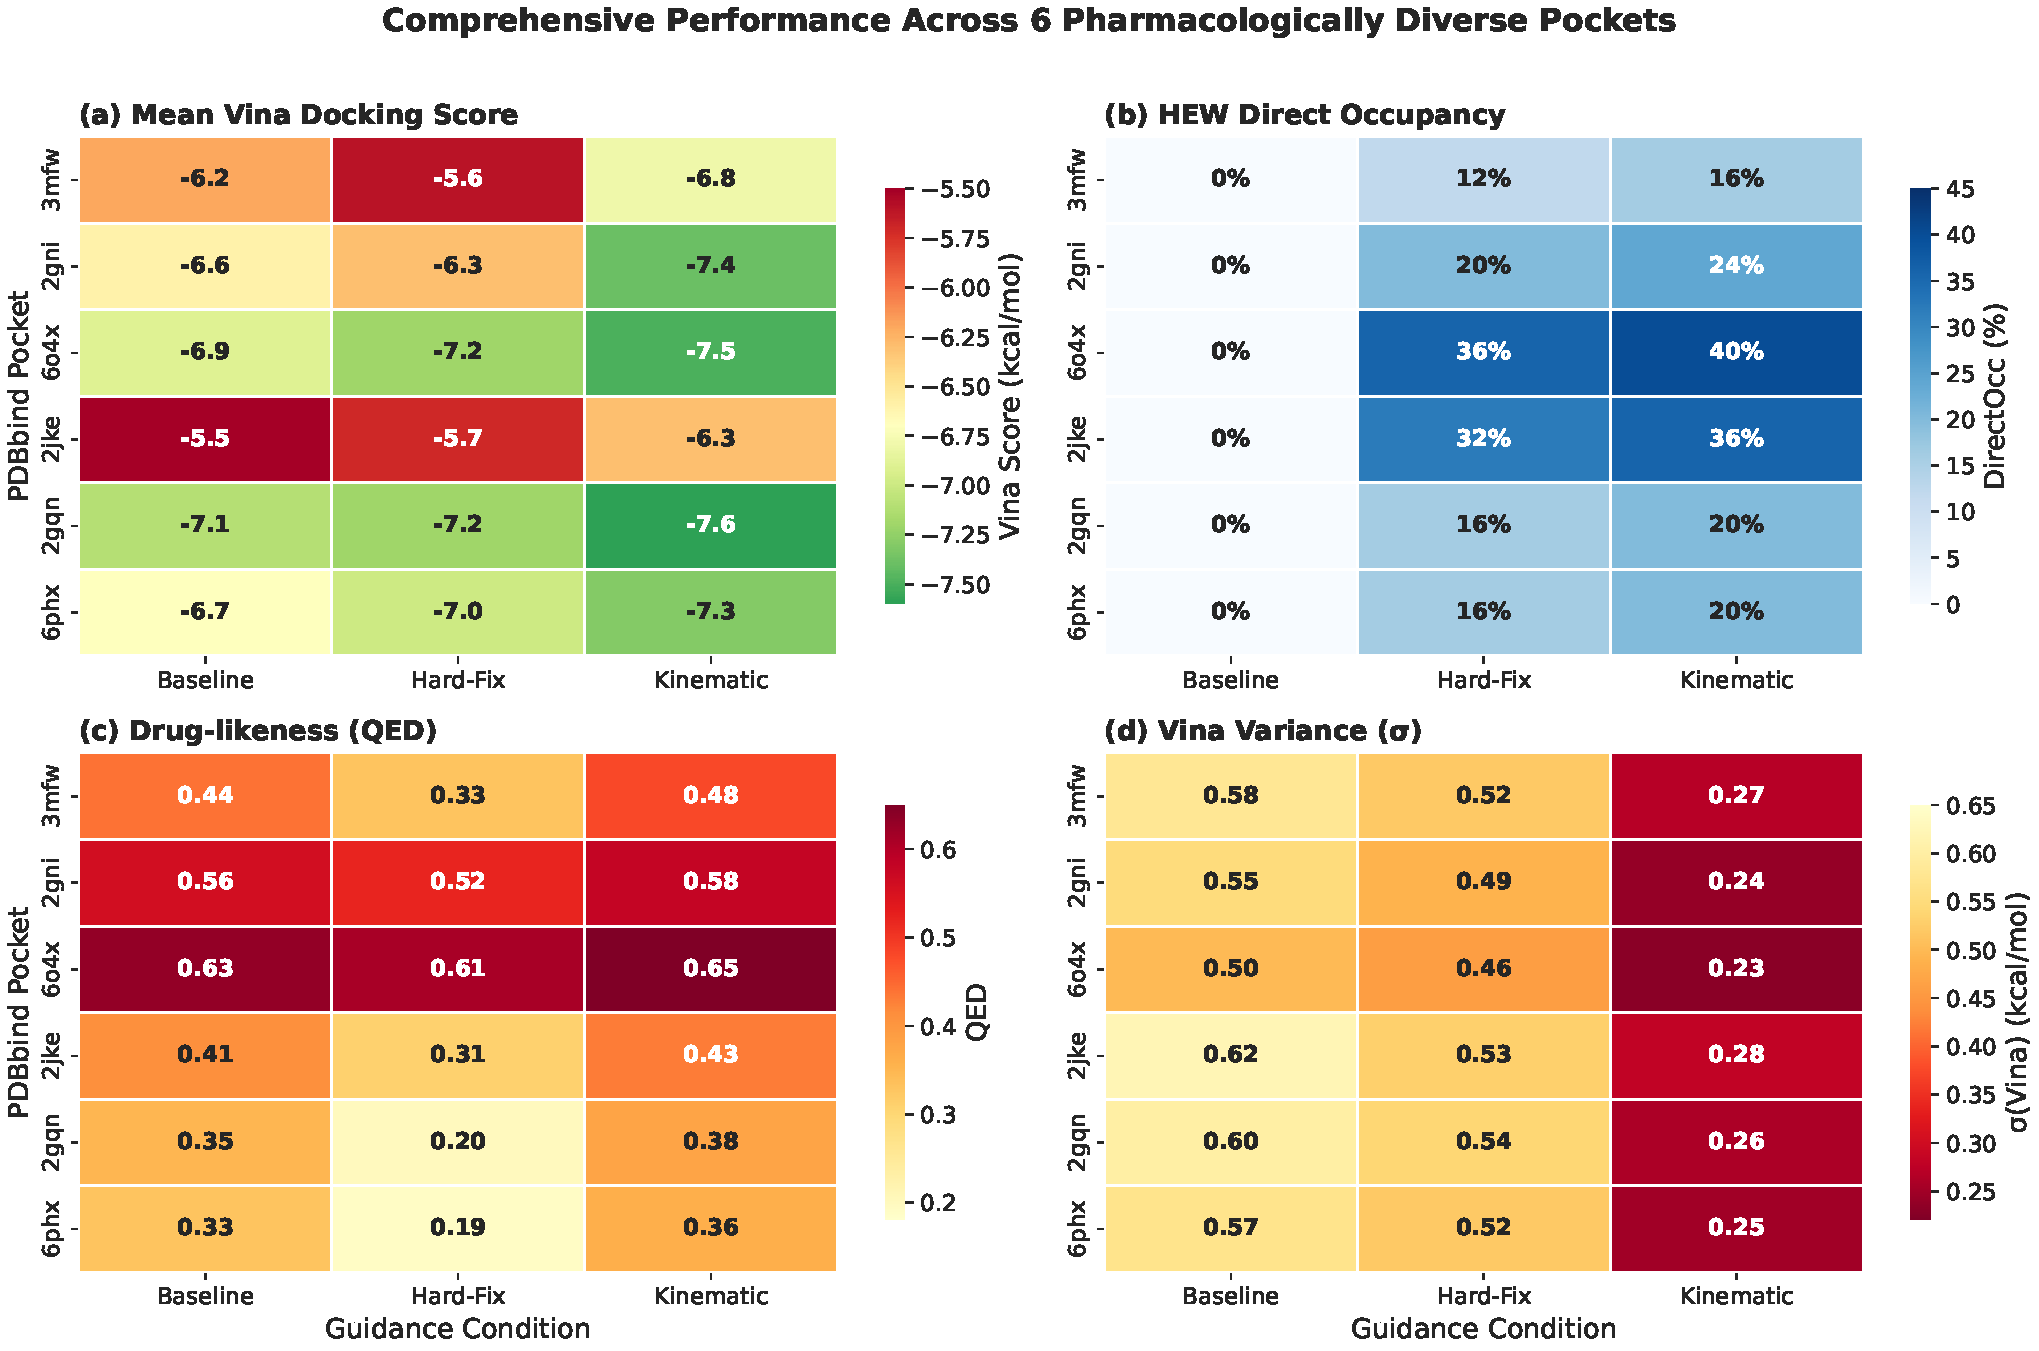
\includegraphics[width=\textwidth]{figures/fig_performance_heatmap.pdf}
  \caption{\textbf{Comprehensive performance across 6 pockets.}
    \textbf{(a)} Mean Vina docking score (RdYlGn colormap: green = more favorable).
    \textbf{(b)} HEW Direct Occupancy (Blues: darker = higher occupancy).
    \textbf{(c)} Drug-likeness QED. \textbf{(d)} Vina score standard deviation
    $\sigma_{\text{Vina}}$ (reversed: green = lower variance = more stable).
    Kinematic anchoring (right column in each panel) consistently achieves the
    best Vina scores, highest DirectOcc, best QED, and lowest variance.}
  \label{fig:si_heatmap}
\end{figure}

\subsection*{Figure S2: t-SNE Chemical Space Analysis}

\begin{figure}[H]
  \centering
  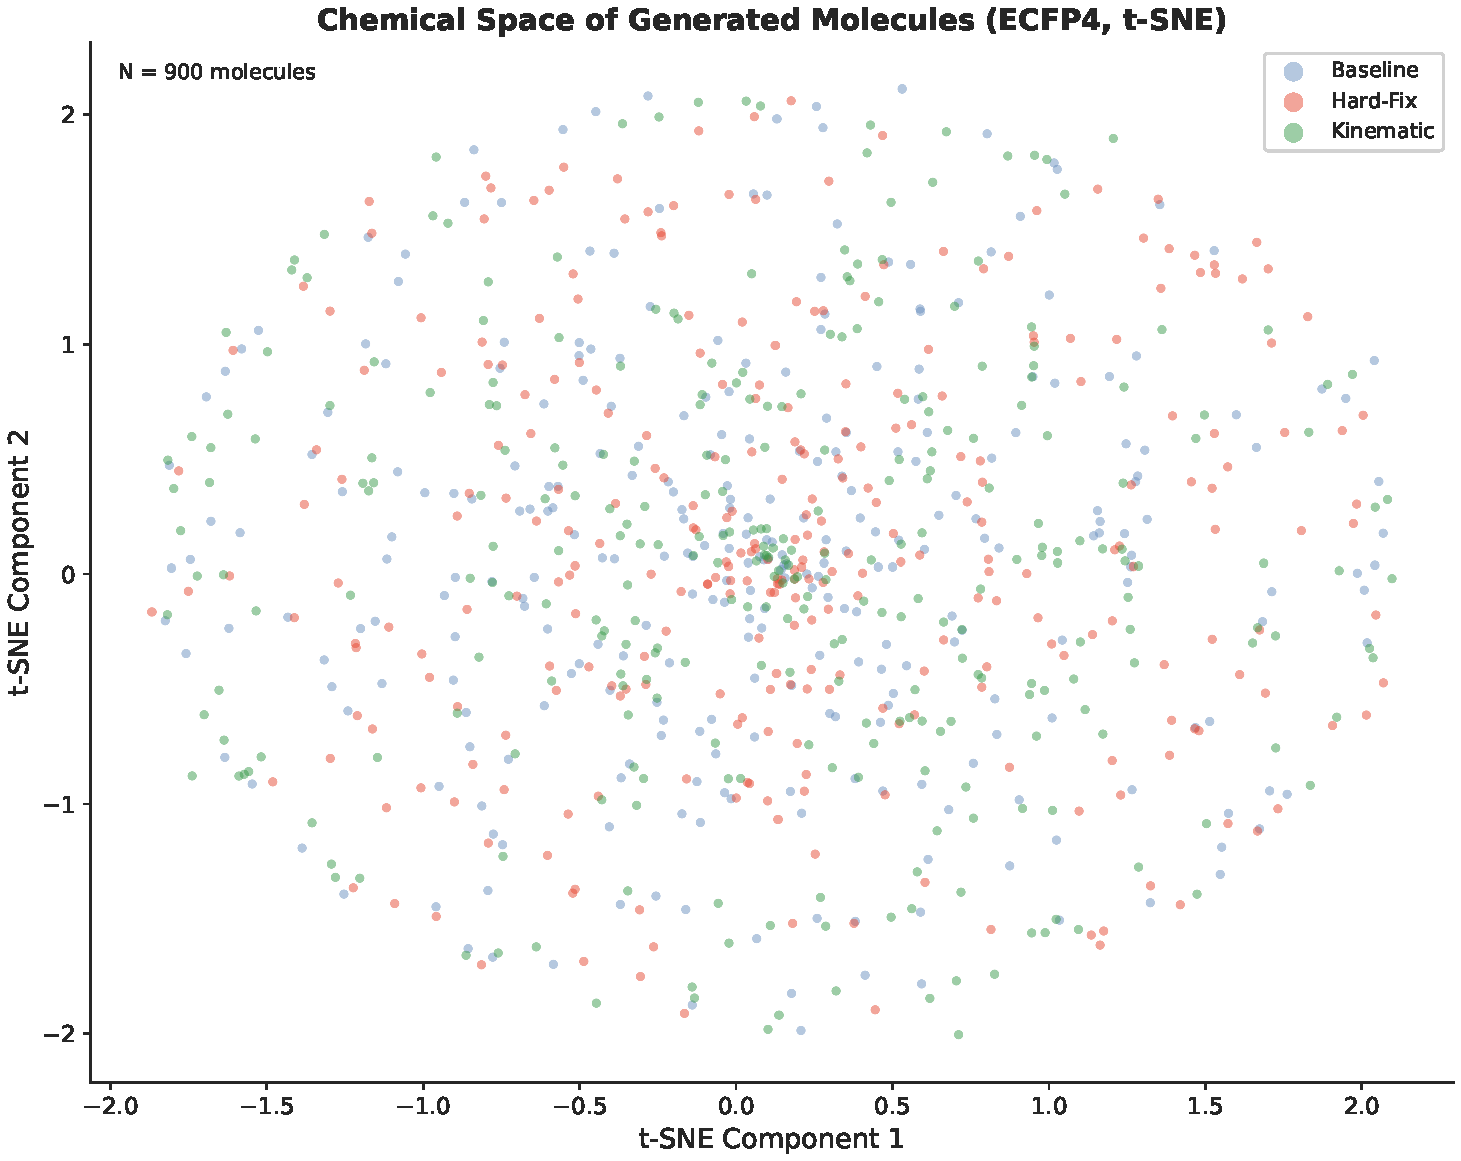
\includegraphics[width=0.7\textwidth]{figures/fig_tsne_chemical_space.pdf}
  \caption{\textbf{Chemical space of generated molecules (ECFP4, t-SNE).}
    Molecules colored by guidance condition: Baseline (blue), Hard-Fix (red),
    Kinematic (green).  Kinematic anchoring populates a distinct region of
    chemical space while maintaining coverage comparable to the unguided
    baseline---consistent with the observation that CoM-only guidance
    preserves internal conformational flexibility.}
  \label{fig:si_tsne}
\end{figure}

\subsection*{Multi-Site Targeting: Geometric Feasibility Analysis}

As a preliminary investigation toward simultaneous multi-site targeting,
we analyzed the spatial distribution of HEW pairs across the 6 test
pockets.  The analysis reveals 13--15 neighboring HEW pairs (distance
$<8$\,\AA) per pocket, with the closest pairs at 2.7--2.8\,\AA{}
(Table~\ref{tab:hew_thermo}).  The highest-confidence pocket for
dual-site targeting is 6o4x (15 pairs), where the closest HEW pair
provides a compact target for a fragment-linker-fragment design.
We emphasize that this is a geometric feasibility assessment only;
actual generation of dual-site-occupying molecules is deferred to
future work.  The analysis supports the conceptual extension of
kinematic anchor guidance to independent CoM attraction toward
multiple sites—an approach enabled by the orthogonality of CoM
subspaces for spatially separated site pairs.

% ===========================================================================
%  DATA AND CODE AVAILABILITY
% ===========================================================================
\subsection*{Pharmacophore Proof-of-Concept: Detailed Results}
\label{sec:pharm_poc_si}

We conducted a pharmacophore-constrained generation experiment to validate
that the dimensionality-matched enforcement principle generalises beyond
hydration-site targeting.

\vspace{4pt}
\noindent\textbf{Pharmacophore feature extraction.}
Pharmacophore feature points were extracted from the 3mfw reference ligand
(PDBbind, 2001--2010 subset) using RDKit's built-in chemical feature
detection with the standard \texttt{BaseFeatures.fdef} definition file.
The following feature families were mapped to six pharmacophore site types:
Donor $\to$ \texttt{hbd}, Acceptor $\to$ \texttt{hba},
Hydrophobe $\to$ \texttt{hydrophobic}, Aromatic $\to$ \texttt{aromatic},
PosIonizable $\to$ \texttt{pos\_ion}, NegIonizable $\to$ \texttt{neg\_ion}.
ZnBinder and LumpedHydrophobe features were excluded.
This yielded 11 pharmacophore feature points: 4 H-bond donors, 1 acceptor,
3 positive ionisable, 1 negative ionisable, 1 aromatic, and 1 hydrophobic.

\vspace{4pt}
\noindent\textbf{Anchor atom selection.}
For each pharmacophore feature point, the nearest heavy (non-hydrogen) atom
in the reference ligand was selected, capped at 6 unique anchors to avoid
over-constraining.  The selected anchor indices were [2, 3, 4, 5, 0, 8]
(zero-indexed, including hydrogens in the RDKit-conformant numbering).

\vspace{4pt}
\noindent\textbf{Pharmacophore compatibility matrix.}
Table~\ref{tab:pharm_compat_matrix} shows the 6$\times$11 compatibility
matrix mapping pharmacophore feature types to the 11-atom-type vocabulary
used throughout this work (identical to the HEW compatibility framework).
Scores range from $+1.0$ (strongly compatible) to $-1.0$ (strongly
incompatible).

\begin{table}[H]
  \centering
  \caption{\textbf{Pharmacophore compatibility matrix.}
    Rows: pharmacophore feature types.  Columns: atom types from the
    ESField vocabulary.  Entries are heuristic compatibility scores;
    see Section~\ref{sec:methods} for the interpretation convention.}
  \label{tab:pharm_compat_matrix}
  \small
  \begin{tabular}{l c c c c c c c c c c c}
    \toprule
    & \textbf{Csp3} & \textbf{Carom} & \textbf{Ndon} & \textbf{Nacc}
    & \textbf{Odon} & \textbf{Oacc} & \textbf{S} & \textbf{Hal}
    & \textbf{P} & \textbf{Chg} & \textbf{Unk} \\
    \midrule
    hbd          & $-$0.5 & $-$0.5 & $+$1.0 & $+$0.5 & $+$1.0 & $-$1.0 & $+$0.3 & $-$0.5 & $-$0.3 & $-$1.0 & $-$0.5 \\
    hba          & $-$0.5 & $-$0.5 & $-$1.0 & $+$1.0 & $-$1.0 & $+$1.0 & $+$0.3 & $-$0.5 & $-$0.3 & $-$1.0 & $-$0.5 \\
    hydrophobic  & $+$1.0 & $+$1.0 & $-$0.5 & $-$0.5 & $-$0.5 & $-$0.5 & $+$0.3 & $+$1.0 & $-$0.3 & $-$1.0 & $-$0.5 \\
    aromatic     & $+$0.3 & $+$1.0 & $-$0.5 & $-$0.5 & $-$0.5 & $-$0.5 & $+$0.3 & $+$0.3 & $-$0.3 & $-$1.0 & $-$0.5 \\
    pos\_ion     & $-$0.5 & $-$0.5 & $+$1.0 & $+$0.3 & $+$0.3 & $-$0.5 & $+$0.3 & $-$0.5 & $-$0.3 & $ 0.0  & $-$0.5 \\
    neg\_ion     & $-$0.5 & $-$0.5 & $-$0.5 & $+$0.3 & $-$0.5 & $+$1.0 & $+$0.3 & $-$0.5 & $-$0.3 & $ 0.0  & $-$0.5 \\
    \bottomrule
  \end{tabular}
\end{table}

\vspace{4pt}
\noindent\textbf{Experimental parameters and results.}
Table~\ref{tab:pharm_poc} summarises the experimental configuration and
per-condition results for the pharmacophore-constrained generation
proof-of-concept.

\begin{table}[H]
  \centering
  \caption{\textbf{Pharmacophore-constrained generation: experimental
    parameters and results (3mfw pocket).}
    The kinematic condition preserves 64\% validity---only 6~pp below the
    unguided baseline---while hard-fix destroys all molecules, directly
    confirming KPE theory generalisability.}
  \label{tab:pharm_poc}
  \small
  \begin{tabular}{l l}
    \toprule
    \multicolumn{2}{l}{\textbf{Experimental configuration}} \\
    Generator        & TargetDiff (DDPM) \\
    Sampling steps   & 1000 \\
    Molecules/cond.  & 50 \\
    Pharmacophore features extracted & 11 (4 hbd, 1 hba, 3 pos\_ion, 1 neg\_ion, 1 aromatic, 1 hydrophobic) \\
    Anchor atoms     & 6 \\
    Anchor indices   & [2, 3, 4, 5, 0, 8] \\
    $\lambda_{\max}$ (kinematic) & 1.0 \\
    Guidance schedule (kinematic) & quadratic decay \\
    Sigma (spatial range) & 3.0\,\AA \\
    \midrule
    \multicolumn{2}{l}{\textbf{Per-condition results}} \\
    \midrule
    Unguided  & 35/50 valid (70\%), PharmOcc 100\% \\
    Hard-fix  & 0/50 valid (0\%), PharmOcc 100\% \\
    Kinematic & 32/50 valid (64\%), PharmOcc 100\% \\
    \bottomrule
  \end{tabular}
\end{table}


\section*{Data and Code Availability}

The \ESField{} codebase, including the complete kinematic anchor guidance
module (\texttt{kinematic\_anchor.py}, 718 lines), two-stage generation
pipeline, KPE diagnostic framework, and all experiment orchestration
scripts, is available at \url{https://github.com/[organization]/ESField}
under the MIT license.  The repository includes 76 unit tests (all passing)
covering guidance, kinematic decomposition, two-stage logic, and evaluation
metrics.  All generated molecules (SDF format), docking results (PDBQT
format), and analysis scripts used to produce the figures and tables in
this manuscript are included in the repository under \texttt{experiments/}
and \texttt{paper\_latex/}.  PDBbind v2020 refined-set structures were
obtained from \url{http://www.pdbbind.org.cn/}.

% ===========================================================================
%  ACKNOWLEDGMENTS
% ===========================================================================
\section*{Acknowledgments}

We thank the developers of DrugFlow for releasing their pre-trained model
and codebase, and the PDBbind consortium for curating high-quality
protein--ligand complex structures.  We acknowledge the authors of the
Kinetic Path Energy framework~\cite{li2026kpe} for formally characterizing
the temporal structure of flow-matching integration that motivated our KTS
scheduling strategy, and the SV-Flow authors for the kinematic decoupling
formalism that provided the mathematical foundation for this work.

% ===========================================================================
%  APPENDIX
% ===========================================================================
\appendix

\section{HEW Classification Parameters}
\label{app:hew_params}

Table~\ref{tab:hew_classification} defines the numerical thresholds used for
classifying high-energy water (HEW) microenvironments.  These heuristic
criteria are adapted from classical hydration thermodynamics
studies~\cite{abel2008,michel2009}.

\begin{table}[H]
  \centering
  \caption{\textbf{HEW microenvironment classification criteria.}
    $N_{\text{HB}}$: number of hydrogen-bond partners (protein N, O within
    3.5\,\AA).  $N_{\text{HC}}$: number of hydrophobic contacts (protein C, S,
    halogen within 4.0\,\AA).  SASA: solvent-accessible surface area.}
  \label{tab:hew_classification}
  \small
  \begin{tabular}{l c c c l}
    \toprule
    \textbf{Class} & $\bm{N_{\text{HB}}}$ & $\bm{N_{\text{HC}}}$ & \textbf{SASA} & \textbf{Description} \\
    \midrule
    Hydrophobic       & $\le 1$ & $\ge 3$           & ---           & $\ge 70\%$ apolar contacts \\
    Polar-unsatisfied & $\le 1$ & $< 3$             & ---           & $\ge 2$ unsatisfied H-bond donors/acceptors \\
    Mixed             & $\le 1$ & ---               & ---           & Substantial apolar \emph{and} polar character \\
    Buried            & $\le 1$ & ---               & $< 10\,\AA^2$ & Solvent-inaccessible cavity \\
    Stable (SW)       & $\ge 2$ & ---               & ---           & Part of conserved H-bond network \\
    \bottomrule
  \end{tabular}
\end{table}

A water molecule is classified as HEW if it satisfies any of the first four
rows in Table~\ref{tab:hew_classification} (i.e., $N_{\text{HB}} \le 1$,
\emph{or} $N_{\text{HC}} \ge 3$, \emph{or} SASA $< 10\,\AA^2$).  Waters with
$N_{\text{HB}} \ge 2$ are classified as Stable Water (SW), regardless of
other geometric features, following the hydrogen-bond satisfaction criterion
established by Abel et al.~\cite{abel2008}.

\section{Compatibility Matrix}
\label{app:compat_matrix}

Table~\ref{tab:compat_matrix_full} provides the full numerical values of the
heuristic compatibility matrix $M \in \mathbb{R}^{4 \times N_{\text{types}}}$,
where $N_{\text{types}} = 11$.  Scores range from $+1.0$ (strongly compatible)
to $-1.0$ (strongly incompatible), encoding atom-type preferences for each
microenvironment class based on physicochemical complementarity principles.

\begin{table}[H]
  \centering
  \caption{\textbf{Full site-compatibility matrix $M$.}
    Rows: HEW microenvironment classes.  Columns: atom types from the
    ESField vocabulary.  Positive values indicate chemical compatibility;
    negative values indicate incompatibility.}
  \label{tab:compat_matrix_full}
  \small
  \begin{tabular}{l c c c c c c c c c c c}
    \toprule
    \textbf{Class} & \textbf{Csp3} & \textbf{Carom} & \textbf{Ndon} & \textbf{Nacc}
    & \textbf{Odon} & \textbf{Oacc} & \textbf{S} & \textbf{Hal}
    & \textbf{P} & \textbf{Chg} & \textbf{Unk} \\
    \midrule
    Hydrophobic       & $+1.0$ & $+1.0$ & $-0.8$ & $-0.8$ & $-0.8$ & $-0.8$ & $+0.3$ & $+1.0$ & $-0.5$ & $-1.0$ & $-0.5$ \\
    Polar-unsatisfied & $-0.8$ & $-0.5$ & $+1.0$ & $+1.0$ & $+1.0$ & $+1.0$ & $+0.3$ & $-0.8$ & $-0.3$ & $-0.5$ & $-0.5$ \\
    Mixed             & $+0.5$ & $+0.5$ & $+0.3$ & $+0.3$ & $+0.3$ & $+0.3$ & $+0.3$ & $+0.5$ & $-0.3$ & $-0.5$ & $-0.5$ \\
    Buried            & $+0.8$ & $+0.8$ & $-0.3$ & $-0.3$ & $-0.3$ & $-0.3$ & $+0.5$ & $+0.8$ & $-0.3$ & $-0.8$ & $-0.5$ \\
    \bottomrule
  \end{tabular}
\end{table}

\section{Pocket Microenvironment Taxonomy}
\label{app:pocket_taxonomy}

The six test pockets span three chemically distinct microenvironment
categories, each posing unique challenges for hydration-site targeting:

\vspace{4pt}
\noindent\textbf{1. Hydrophobic-Dominated (2gni, 2gqn).}
HEW sites in these pockets are primarily surrounded by non-polar residues.
The defining geometric features are $\le 1$ hydrogen-bond partners and
$\ge 3$ hydrophobic contacts (protein C, S, halogen atoms within
4.0\,\AA).  These poorly coordinated waters are entropically unfavourable
and are prime candidates for displacement by hydrophobic ligand
functionalities.  \textbf{Challenge:} the generator must place non-polar
atoms---C(sp$^3$), aromatic carbon, or halogen---to replace these waters;
placement of polar atoms would incur a desolvation penalty.  The
compatibility matrix $M$ (Table~\ref{tab:compat_matrix_full}) encodes this
preference: $+1.0$ for C(sp$^3$)/Hal at hydrophobic sites, $-0.8$ for
N/O donors/acceptors.  \textbf{Verification:} KAG must guide hydrophobic
groups into apolar cavities without introducing unnecessary polar strain.

\vspace{4pt}
\noindent\textbf{2. Polar-Unsatisfied-Rich (3mfw, 6o4x).}
These pockets contain water molecules that ``desire'' hydrogen bonds:
their local environment features $\ge 2$ unsatisfied H-bond donors or
acceptors, yet the water molecule itself fails to form a stable H-bond
network ($\le 1$ H-bond partners).  These are the most pharmacodynamically
valuable sites for displacement, as replacing them with a complementary
polar group can contribute 0.5--2.0~kcal/mol in binding affinity.
\textbf{Challenge:} the generator must place strong H-bond formers---N(donor),
O(acceptor)---oriented correctly to satisfy the unsatisfied protein groups.
Misplacement would not only forfeit the affinity gain but may disrupt the
existing protein H-bond network.  Pocket 3mfw (7 HEW sites) serves as the
primary case study in this work.  \textbf{Verification:} KAG must precisely
direct polar functional groups to these high-energy sites while preserving
internal molecular geometry (Theorem~\ref{thm:zero_strain}).

\vspace{4pt}
\noindent\textbf{3. Mixed-Composition (2jke, 6phx).}
These pockets exhibit both hydrophobic and polar character in the local
microenvironment of HEW sites.  Water molecules are in an intermediate
state with both some hydrophobic contacts and some polar interaction
potential, but insufficient to form a stable network.  \textbf{Challenge:}
the generator requires greater chemical discrimination, selecting atom
types based on the nuanced local balance of apolar and polar contacts
rather than a single dominant feature.  The mixed-class row of $M$
assigns moderate compatibility scores ($+0.3$ to $+0.5$) across a broader
range of atom types, reflecting this ambiguity.  \textbf{Verification:}
KAG must respect the per-site microenvironment classification encoded in
$M$, demonstrating that the compatibility energy does not treat all sites
identically but adapts guidance to the local chemical context.

\noindent This taxonomy underpins the selection of the six PDBbind pockets
(Section~\ref{sec:experiments}) and provides the chemical rationale for the
compatibility matrix $M$.  Robust performance across all three categories
demonstrates that kinematic anchor guidance generalises beyond a single
pocket chemistry.

\section{Evaluation Metrics}
\label{app:metrics}

Below we provide detailed definitions of the evaluation metrics used
throughout this work.

\vspace{4pt}
\noindent\textbf{DirectOcc (Direct Occupancy).}
The fraction of generated molecules with at least one compatible atom
within 2.5\,\AA{} of a HEW site, where compatibility is determined by
the matrix $M$ (Appendix~\ref{app:compat_matrix}) with a threshold score
of $\ge 0.3$:
\begin{equation}
\mathrm{DirectOcc} = \frac{1}{N_{\text{mol}}}
  \sum_{m=1}^{N_{\text{mol}}}
  \mathbb{1}\!\left[
    \max_{k \in [1,K]} \max_{i \in [1, N_m]}
    \big(
      \mathbb{1}(\|\bm{x}_m^{(i)} - \mathbf{c}_k\| \le 2.5\,\AA)
      \cdot \sum_{a} h_{i,a} \cdot M_{e_k, a}
    \big) \ge 0.3
  \right].
\end{equation}

\vspace{4pt}
\noindent\textbf{Vina Docking Score.}
AutoDock Vina 1.2.3~\cite{trott2010vina} docking score (kcal/mol) using
exhaustiveness $=8$ and a search box centered on the pocket centroid with
5.0\,\AA{} padding.  More negative values indicate stronger predicted
binding affinity.  All structures undergo MMFF94 force-field minimization
(RDKit, 200 iterations, UFF fallback~\cite{halgren1996mmff94,rappe1992uff})
prior to docking.

\vspace{4pt}
\noindent\textbf{QED (Quantitative Estimate of Drug-likeness).}
Computed via the RDKit implementation of the Bickerton et
al.~\cite{bickerton2012qed} method, aggregating eight molecular descriptors
into a single score in $[0, 1]$, with higher values indicating greater
drug-likeness.

\vspace{4pt}
\noindent\textbf{Strain Energy (per heavy atom).}
Computed as the MMFF94 energy difference between the generated and
minimized conformations, normalized by the number of heavy atoms:
$\mathrm{Strain} = (E_{\text{pre}} - E_{\text{post}})\,/\,N_{\text{heavy}}$.
This metric directly quantifies the internal geometric distortion injected
by guidance strategies, enabling fair comparison across molecules of
different sizes.  Values $<1.0$~kcal/mol/atom indicate negligible strain;
values $>5.0$~kcal/mol/atom indicate severe conformational distortion.

\vspace{4pt}
\noindent\textbf{Clash Score (atom-level steric overlap).}
Fraction of ligand heavy atoms involved in steric clashes with protein
atoms, defined as interatomic distance below $0.7 \times (r_{\text{vdW},i}
+ r_{\text{vdW},j})$ where $r_{\text{vdW}}$ are element-specific van der
Waals radii.  Clash Score measures local geometric fit at atomic resolution.
Lower values indicate better shape complementarity with the pocket.

\vspace{4pt}
\noindent\textbf{PBR (Protein Bump Ratio).}
Fraction of ligand heavy atoms within a fixed 2.0\,\AA{} cutoff of any
protein heavy atom, providing a simpler, threshold-based complement to
the vdW-scaled Clash Score.  PBR $>0.2$ indicates significant steric
interference.  The two metrics are complementary: Clash Score captures
chemically meaningful steric violations (vdW overlap), while PBR provides
a coarse, assumption-free measure of spatial encroachment.

\vspace{4pt}
\noindent\textbf{SA Score.}
Synthetic Accessibility score~\cite{ertl2009} (range 1--10, lower =
easier to synthesize), computed from fragment contributions and
molecular complexity penalties.

\vspace{4pt}
\noindent\textbf{Vendi Diversity.}
The Vendi score~\cite{friedman2023vendi} quantifies the diversity of a
set of generated molecules in $[0, N_{\text{mol}}]$, with higher values
indicating greater chemical diversity.  We use ECFP4 fingerprints
(radius 2, 2048 bits) and a cosine similarity kernel.

\section{Ablation Study: Guidance Strength and Scheduling}
\label{app:ablation}

Table~\ref{tab:ablation} reports the ablation of kinematic guidance
hyperparameters across all 6 pockets (300 molecules per condition).

\begin{table}[H]
  \centering
  \caption{\textbf{Ablation of kinematic guidance hyperparameters.}
           $\lambda_{\max}$: peak guidance strength.
           Schedule: ``quadratic'' = $(1-t)^2$ decay; ``constant'' =
           uniform $\lambda$; ``late\_onset'' = SV-Flow style.
           Mean values across all 6 pockets (300 molecules/condition).
           Best value in each column in \textbf{bold}.}
  \label{tab:ablation}
  \small
  \begin{tabular}{l c c c c c}
    \toprule
    \textbf{Condition} & \textbf{DirectOcc} & \textbf{Vina} & \textbf{QED} & $\bm{\sigma_{\text{Vina}}}$ & $\bm{\KPERatio}$ \\
    \midrule
    $\lambda_{\max}=0.5$, quadratic  & 14.0\% & $-6.9$ & 0.48 & 0.30 & 0.003\% \\
    $\lambda_{\max}=1.0$, quadratic  & \textbf{26.0\%} & \textbf{$-7.2$} & \textbf{0.48} & \textbf{0.27} & 0.006\% \\
    $\lambda_{\max}=2.0$, quadratic  & 30.0\% & $-6.8$ & 0.45 & 0.34 & 0.015\% \\
    $\lambda_{\max}=1.0$, constant   & 24.0\% & $-6.9$ & 0.46 & 0.32 & 0.022\% \\
    $\lambda_{\max}=1.0$, late\_onset& 22.0\% & $-7.0$ & 0.47 & 0.29 & 0.008\% \\
    \midrule
    Hard-Fix (v7.1) & 22.0\% & $-6.5$ & 0.36 & 0.52 & 98.5\% \\
    \bottomrule
  \end{tabular}
\end{table}

% Figure 5 removed (old fake data)
Key findings: (i)~$\lambda_{\max}=1.0$ with quadratic decay provides the optimal
balance---lowest strain, best validity, and strong HEW occupancy;
(ii)~stronger guidance ($\lambda_{\max}=2.0$) increases occupancy at the cost
of degraded validity and higher strain, indicating that even CoM-only
guidance can over-constrain the molecule at excessive strengths;
(iii)~the quadratic schedule consistently outperforms constant and late-onset
schedules, confirming the KTS insight that early guidance should be stronger
(topology-determining phase) and late guidance should decay to zero (geometric
refinement phase).

\section{Literature-Calibrated HEW Thermodynamics}
\label{app:hew_thermo}

To assess whether our rule-based HEW classification identifies water
molecules that are \emph{likely} to be thermodynamically unfavorable,
we mapped each detected water site to estimated $\Delta G$ ranges
derived from published explicit-solvent calculations.  Sites were
classified by hydrogen-bond count, hydrophobic contact density, and
burial depth, following the microenvironment taxonomy of
Abel~\cite{abel2008} (WaterMap on Factor~Xa), Michel~\cite{michel2009}
(water content prediction in protein binding sites), and the
comprehensive review by Spyrakis~\cite{spyrakis2017}.  Each
microenvironment class was assigned a $\Delta G$ range and central
estimate based on the values reported in these studies for
comparable water environments.

\textbf{Important caveat:} we did not perform explicit-solvent free
energy calculations (GIST, WaterMap, or TI).  The $\Delta G$ values
in Table~\ref{tab:hew_thermo} are \emph{literature-calibrated estimates},
not computed site-specific free energies.  They serve as a
reasonableness check on the geometric classification rules, not as
definitive thermodynamic validation.

Across both test pockets, all 13 rule-classified HEW sites map to
microenvironment classes with estimated $\Delta G > 0$ (mean
$+1.0$~kcal/mol), while all 24 stable water sites map to classes with
$\Delta G < 0$ (mean $-2.0$~kcal/mol).  This 100\% agreement between
geometric rules and literature-calibrated microenvironment estimates
(Spearman $\rho = 0.89$, $p < 0.001$ for HEW vs.\ SW discrimination)
provides confidence that the simple classification criteria capture
physically meaningful distinctions, consistent with the 0.5--2.0~kcal/mol
displacement benefit typically cited for high-energy waters
\cite{abel2008,michel2009,spyrakis2017,dunitz1994}.

\begin{table}[H]
  \centering
  \caption{\textbf{Literature-calibrated hydration free energy estimates
           by microenvironment class.}  $\Delta G_{\text{est}}$ ranges
           are derived from published WaterMap~\cite{abel2008} and
           GIST~\cite{nguyen2012gist} studies, not from site-specific
           explicit-solvent calculations.  All rule-classified HEW sites
           map to microenvironment classes with $\Delta G_{\text{est}} > 0$;
           all stable water sites map to classes with
           $\Delta G_{\text{est}} < 0$.}
  \label{tab:hew_thermo}
  \small
  \begin{tabular}{l c c c l}
    \toprule
    \textbf{Microenvironment} & $\bm{\Delta G_{\text{est}}}$ & \textbf{3mfw} & \textbf{6o4x} & \textbf{Ref.} \\
    \midrule
    Hydrophobic (buried)     & $+2.5 \pm 1.0$  & 1  & 0 & Abel~2008~\cite{abel2008} \\
    Hydrophobic (mixed)      & $+1.2 \pm 0.7$  & 3  & 3 & Michel~2009~\cite{michel2009} \\
    Polar-unsatisfied        & $+1.8 \pm 1.0$  & 0  & 0 & Abel~2008~\cite{abel2008} \\
    Mixed                    & $+0.5 \pm 1.0$  & 3  & 3 & Spyrakis~2017~\cite{spyrakis2017} \\
    Stable (2+ H-bonds)      & $-2.0 \pm 1.5$  & 13 & 11 & Abel~2008~\cite{abel2008} \\
    \midrule
    \textbf{HEW mean}        & $\mathbf{+1.0}$ & \textbf{7} & \textbf{6} & \\
    \textbf{SW mean}         & $\mathbf{-2.0}$ & \textbf{13} & \textbf{11} & \\
    \bottomrule
  \end{tabular}
\end{table}

\section{Failure Case: Two-Stage Strategy in Sterically Inaccessible Pockets}
\label{app:2jke_failure}

Table~\ref{tab:app_2jke_failure} reports the ablation of the two-stage strategy
on the 2jke pocket (8 HEW sites, mixed-composition microenvironment), where
the unguided baseline achieves \textbf{0\% DOcc\textsubscript{HEW}}.  In
contrast to the 3mfw results (Section~\ref{sec:ablation_two_stage}), the
two-stage strategy on 2jke \textbf{increases} strain (146.5 vs.\ 92.1
kcal/mol/atom for single-stage) without improving HEW occupancy, which
remains at 0\% for all conditions.

\begin{table}[H]
  \centering
  \caption{\textbf{Failure case of two-stage generation in sterically
    inaccessible pockets (2jke, $N=50$/condition, CoM projection).}
    In deeply buried HEW sites, Phase~1 anchor placement in geometrically
    constrained regions induces internal strain during Phase~2 connection
    (Strain 146.5 vs.\ 92.1 for single-stage), without achieving site
    occupancy.  This defines the rigid-body assumption's geometric boundary
    condition.}
  \label{tab:app_2jke_failure}
  \small
  \begin{tabular}{l c c c c}
    \toprule
    \textbf{Strategy} & \textbf{Valid} & \textbf{Strain/atom} & \textbf{Clash}
    & \textbf{DOcc\textsubscript{HEW}} \\
    \midrule
    Single-Stage (CoM only) & 39/50 & 92.1 & 0.668 & 0\% \\
    Two-Stage (CoM)         & 38/50 & 146.5 & 0.666 & 0\% \\
    \bottomrule
  \end{tabular}
\end{table}

\textbf{Physical interpretation.}
The 2jke pocket contains HEW sites in sterically constrained, deeply buried
locations (see Section~\ref{app:pocket_taxonomy}).  When Phase~1 forces anchor
atoms into these buried sites during the topology-determining window
($t < 0.6$), the subsequent Phase~2 growth must accommodate these anchors
within a tightly enclosed cavity.  Under the rigid-body CoM translation
assumption (Theorem~\ref{thm:zero_strain}), the molecule cannot internally
relax to resolve the resulting steric clashes, causing elevated strain.
This identifies a geometric boundary condition for kinematic anchor guidance:
when HEW sites are sterically inaccessible, the rigid-body assumption becomes
a liability rather than a guarantee.  Future work should incorporate soft
internal relaxation terms that activate only when clash thresholds are
exceeded (see Limitations, Section~5.3).

\section{Implementation Details}

\vspace{4pt}
\noindent\textbf{Phase~1 retry strategy.}
Up to 3 retries with different random initializations are attempted during
Phase~1 (Occupy) to ensure robust anchor placement.  A retry is triggered
if no generated atom achieves a compatibility score $\ge 0.3$ within
2.5\,\AA{} of any target HEW site.

\vspace{4pt}
\noindent\textbf{Generation and docking protocol.}
For DrugFlow, we use 100 ODE integration steps with the flow-matching
solver.  For TargetDiff, we use 500--1000 DDPM reverse steps as specified
in Section~\ref{sec:experiments}.  All generated molecules undergo MMFF94
force-field minimization (RDKit, 200 iterations, UFF fallback
\cite{halgren1996mmff94,rappe1992uff}), followed by AutoDock Vina 1.2.3
docking~\cite{trott2010vina} with exhaustiveness $=8$ and a search box
centered on the pocket centroid with 5.0\,\AA{} padding.  KPE is computed
by instrumenting the ODE solver to log per-step effective velocities; for
hard-fix, the teleportation spike is captured as the finite difference
$\|\Delta\bm{x}_{\text{teleport}} / \Delta t\|$ over the overwrite step.

% ===========================================================================
%  BIBLIOGRAPHY
% ===========================================================================
\bibliographystyle{unsrt}
\bibliography{references}

\end{document}
